\section{Fake Data}{}
\label{sec:fakedata}

Five sets of fake data were produced to test the robustness of the analysis.  These fake data sets are treated as if they were real data, and the full analysis flow was performed for each of the sets. All of the selections were examined; including the $\pi^{0}$ selection, 2+ shower sidebands, $\nu_{\mu}$ selection, as well as the inclusive and exclusive, 1eNp and 1e0p, electron neutrino selections.  The muon neutrino and exclusive electron neutrino selections were then passed to SBNFit to perform the constraint of the systematic errors and calculate the sensitivity.  In all cases, except for the muon neutrino selection, where the CRT is used, data from both the run 1 and run 3 samples are combined.

There are a few aspects in which the fake data sets are different than the real data sets. These are noted here.  In particular, there is no EXT or dirt contribution to the fake-data to MC comparison plots, by construction in the way that the fake datasets were produced.  Also, no $\pi^{0}$ scaling is applied to these plots because good scaling agreement is seen out of the box in the $\pi^{0}$ samples. The optical filter is also not applied to events in the fake-data samples.

\subsection{Set 1}

The first selections studied are those rich in $\pi^{0}$s. Fig~\ref{fig:fakedata:set1:pi0} shows the reconstructed $\pi^{0}$ mass for the $\pi^{0}$ selection. Good data-MC agreement is observed, as well as good energy scale resolution in the reconstructed $\pi^{0}$ mass. 
\begin{figure}[H]
\begin{center}
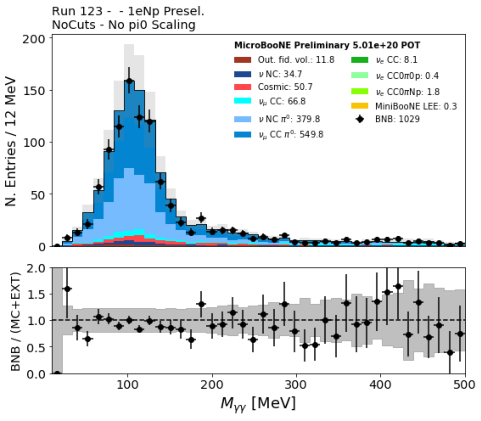
\includegraphics[width=0.45\textwidth]{Fakedata/set1/pi0.pdf}
\caption{\label{fig:fakedata:set1:pi0} $\pi^{0}$ selection.}
\end{center}
\end{figure}

Fig~\ref{fig:fakedata:set1:2shr} shows the 2+ shower side band for the 1eNp and 1e0p selections. There is good agreement in the 2+ shower side band in the 1e0p selection.  There is a slight normalization deficit, within systematic errors, in the 2+ shower side band in the 1eNp selection. 

\begin{figure}[H] 
\begin{center}
    \begin{subfigure}[b]{0.45\textwidth}
    \centering
    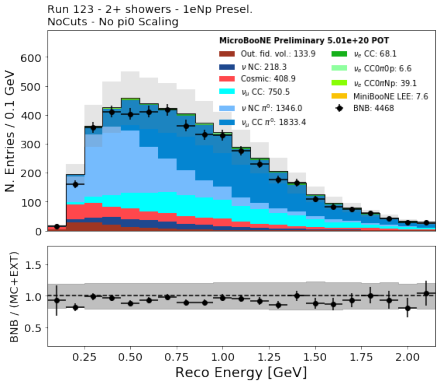
\includegraphics[width=1.00\textwidth]{Fakedata/set1/np_2shr.pdf}
    \caption{\label{fig:fakedata:set1:2shrnp} 1eNp at pre-selection}
    \end{subfigure}
    \begin{subfigure}[b]{0.45\textwidth}
    \centering
    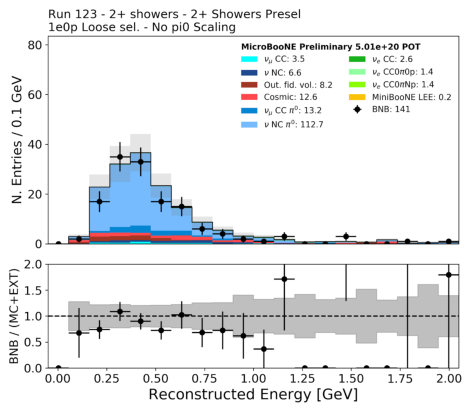
\includegraphics[width=1.00\textwidth]{Fakedata/set1/zp_2shr.pdf}
    \caption{\label{fig:fakedata:set1:2shr0p} 1e0p after loose selection}
    \end{subfigure}
\caption{\label{fig:fakedata:set1:2shr} 2+ shower side bands.}
\end{center}
\end{figure}

The inclusive electron neutrino selection is sensitive to the electron neutrino content in the beam and can also be used to measure data-MC agreement.  Fig~\ref{fig:fakedata:set1:inc_presel} shows the shower dE/dx of the inclusive selection at pre-selection.  The distribution agrees within errors.   

\begin{figure}[H]
\begin{center}
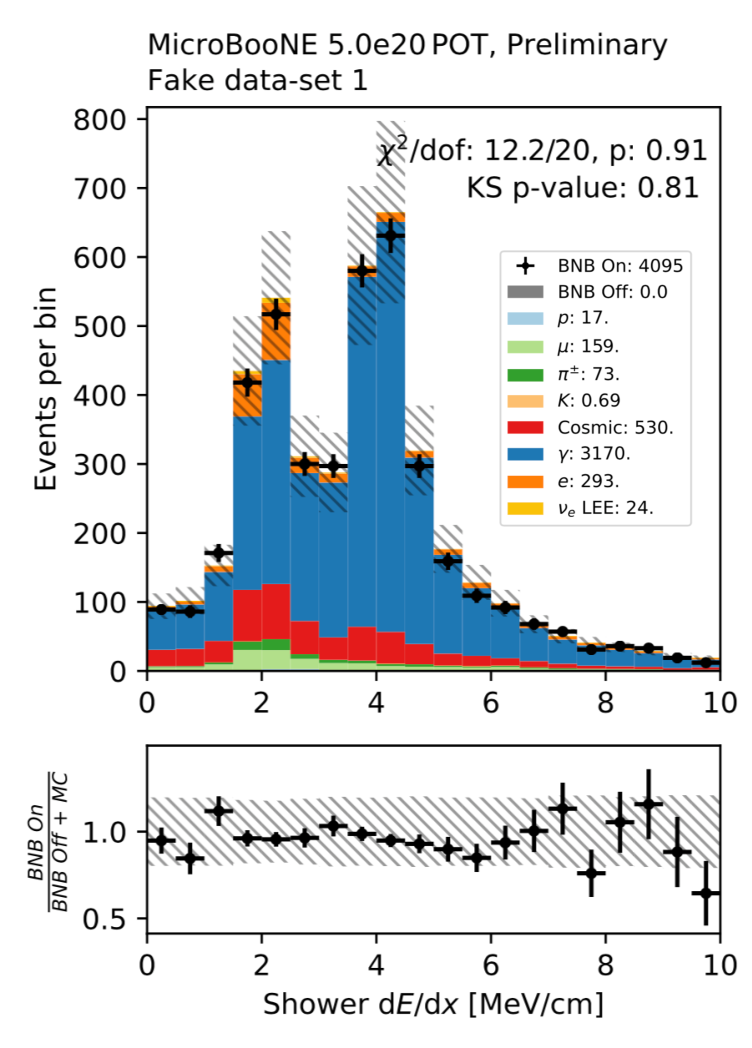
\includegraphics[width=0.45\textwidth]{Fakedata/set1/inc_presel.pdf}
\caption{\label{fig:fakedata:set1:inc_presel} dE/dx of inclusive selection at pre-selection.}
\end{center}
\end{figure}

Fig~\ref{fig:fakedata:set1:inc_postsel} shows the final inclusive selection in electron shower energy, shower theta and track multiplicity.  After selection these distributions agree within errors.

\begin{figure}[H]
\begin{center}
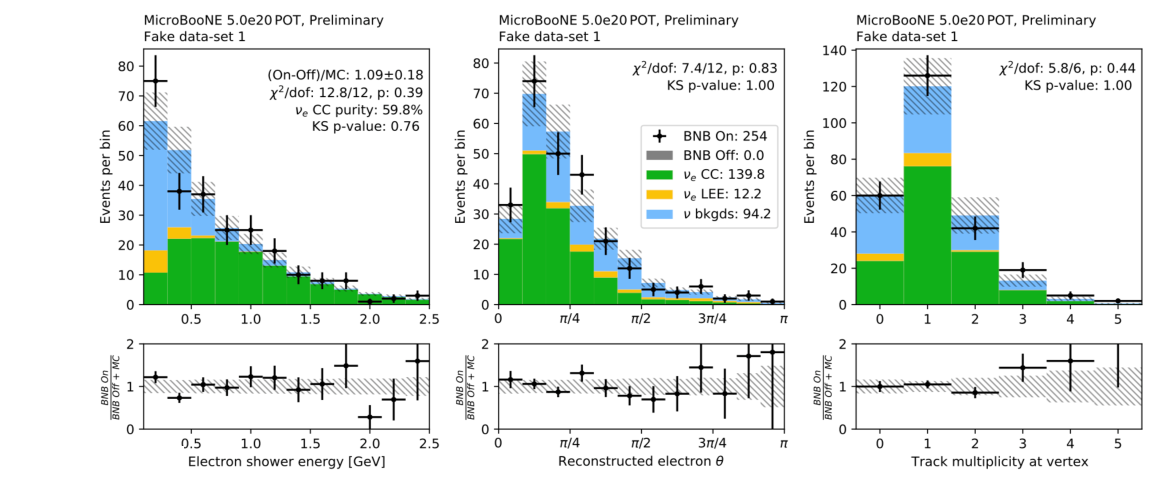
\includegraphics[width=0.9\textwidth]{Fakedata/set1/inc_postsel.pdf}
\caption{\label{fig:fakedata:set1:inc_postsel} Inclusive selection of electron neutrinos. From left to right: electron shower energy, shower theta, track multiplicity.}
\end{center}
\end{figure}

The muon neutrino selection data-MC agreement was also studied in the fake data.  Only the run 3 fake data is used because the CRT is used in the selection. Comparisons where runs 1 and 3 are combined show similar effects to the ones observed here. 
Fig~\ref{fig:fakedata:set1:numu} shows the muon neutrino selection in lepton angle, energy, and total number of tracks. Overall low normalization is observed in most variables in the muon neutrino selection.  This variation is within the systematic uncertainty so that the covariance matrix fit can account for the differences.

\begin{figure}[H] 
\begin{center}
    \begin{subfigure}[b]{0.3\textwidth}
    \centering
    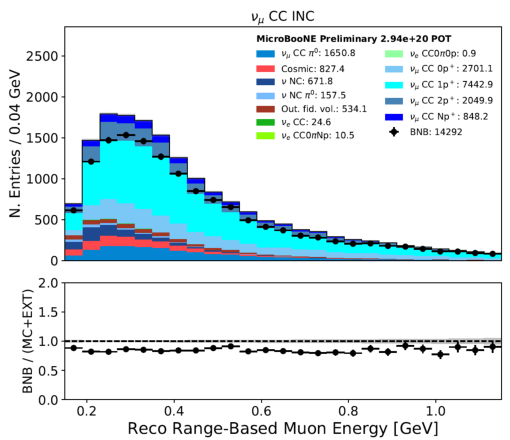
\includegraphics[width=1.00\textwidth]{Fakedata/set1/numu_energy.pdf}
    \caption{\label{fig:fakedata:set1:numu_energy} Energy.}
    \end{subfigure}
    \begin{subfigure}[b]{0.3\textwidth}
    \centering
    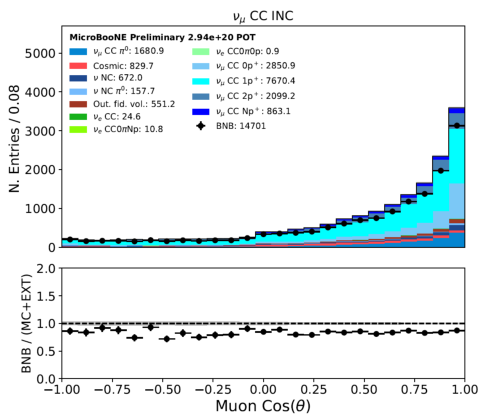
\includegraphics[width=1.00\textwidth]{Fakedata/set1/numu_costheta.pdf}
    \caption{\label{fig:fakedata:set1:numu_costheta} cos($\theta$)}
    \end{subfigure}
    \begin{subfigure}[b]{0.3\textwidth}
    \centering
    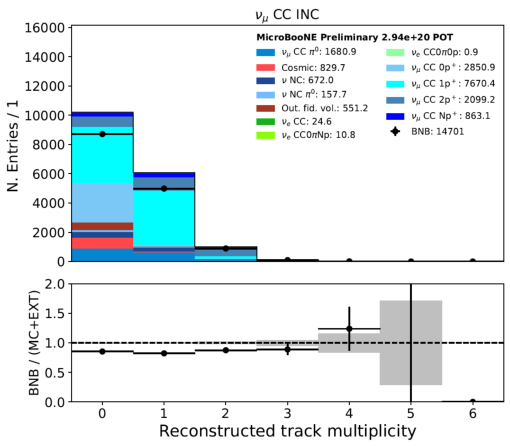
\includegraphics[width=1.00\textwidth]{Fakedata/set1/numu_ntracks.pdf}
    \caption{\label{fig:fakedata:set1:numu_ntracks} Number of tracks}
    \end{subfigure}
\caption{\label{fig:fakedata:set1:numu} Muon neutrino selection. Systematic uncertainties are not plotted, but are included in the constraint.}
\end{center}
\end{figure}

The exclusive electron neutrino selections were also performed on the fake data. Fig~\ref{fig:fakedata:set1:presel} shows the reconstructed energy of events passing the 1eNp and 1e0p pre-selections.  Good agreement is observed in both cases.

\begin{figure}[H] 
\begin{center}
    \begin{subfigure}[b]{0.45\textwidth}
    \centering
    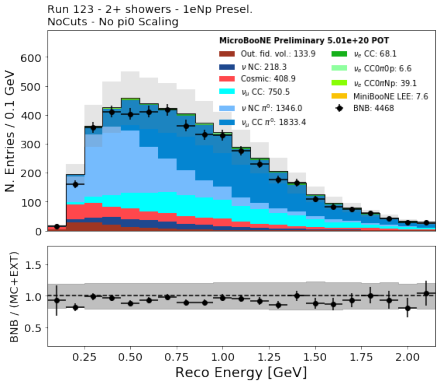
\includegraphics[width=1.00\textwidth]{Fakedata/set1/np_2shr.pdf}
    \caption{\label{fig:fakedata:set1:Np_presel_recoe} 1eNp at pre-selection}
    \end{subfigure}
    \begin{subfigure}[b]{0.45\textwidth}
    \centering
    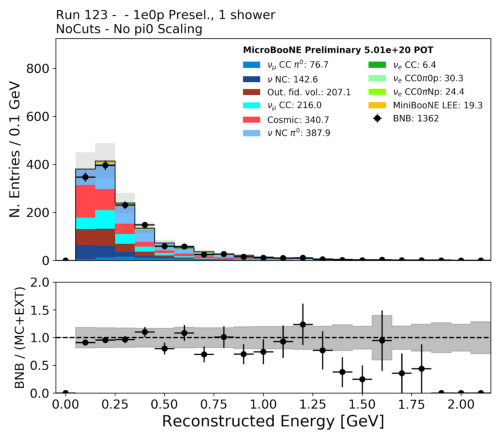
\includegraphics[width=1.00\textwidth]{Fakedata/set1/zp_presel_recoe.pdf}
    \caption{\label{fig:fakedata:set1:2shr0p} 1e0p after pre-selection}
    \end{subfigure}
\caption{\label{fig:fakedata:set1:presel} Exclusive electron neutrino selections at pre-selection stage.}
\end{center}
\end{figure}

Fig~\ref{fig:fakedata:set1:npsel} shows various distributions after the 1eNp BDT selection.  An excess is observed at low reconstructed neutrino energy. There is also an excess in one track events relative to two track events which suggests that there may be some migration between the categories.

\begin{figure}[H] 
\begin{center}
    \begin{subfigure}[b]{0.45\textwidth}
    \centering
    \includegraphics[width=1.00\textwidth]{Fakedata/set1/Np_postsel_recoe.pdf}
    \caption{\label{fig:fakedata:set1:Np_postsel_recoe} Reconstructed energy.}
    \end{subfigure}
    \begin{subfigure}[b]{0.45\textwidth}
    \centering
    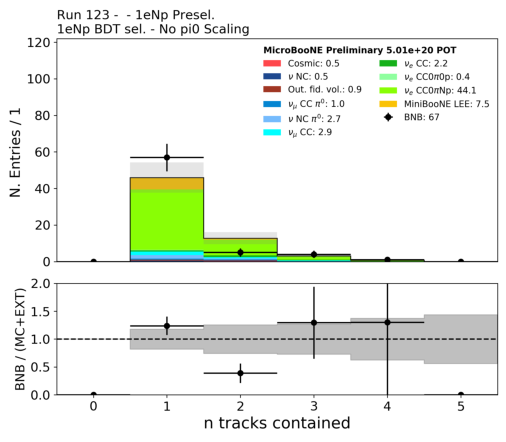
\includegraphics[width=1.00\textwidth]{Fakedata/set1/Np_postsel_ntracks.pdf}
    \caption{\label{fig:fakedata:set1:Np_postsel_ntracks} Number of tracks.}
    \end{subfigure}
\caption{\label{fig:fakedata:set1:npsel} 1eNp BDT selection.}
\end{center}
\end{figure}

Fig~\ref{fig:fakedata:set1:zpsel} shows the 1e0p selection after BDT selection.  An excess is observed at low energy. There is also an excess in high BDT response and in overall normalization.

\begin{figure}[H] 
\begin{center}
    \begin{subfigure}[b]{0.3\textwidth}
    \centering
    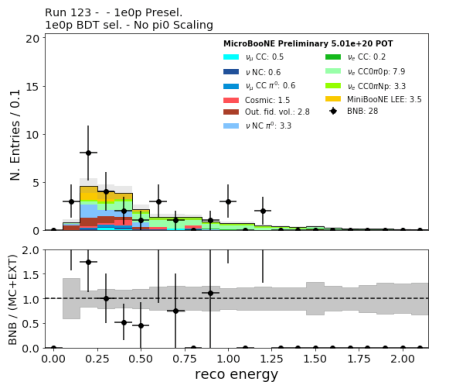
\includegraphics[width=1.00\textwidth]{Fakedata/set1/zp_postsel_recoe.pdf}
    \caption{\label{fig:fakedata:set1:zp_postsel_recoe} Reconstructed energy.}
    \end{subfigure}
    \begin{subfigure}[b]{0.3\textwidth}
    \centering
    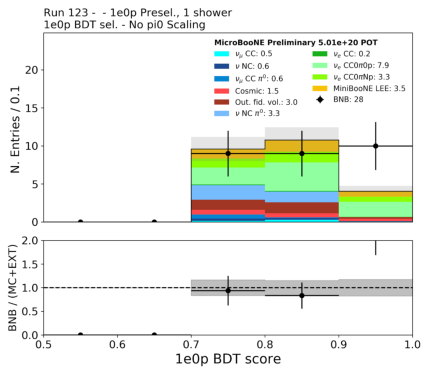
\includegraphics[width=1.00\textwidth]{Fakedata/set1/zp_postsel_bdt.pdf}
    \caption{\label{fig:fakedata:set1:zp_postsel_bdt} BDT response.}
    \end{subfigure}
    \begin{subfigure}[b]{0.3\textwidth}
    \centering
    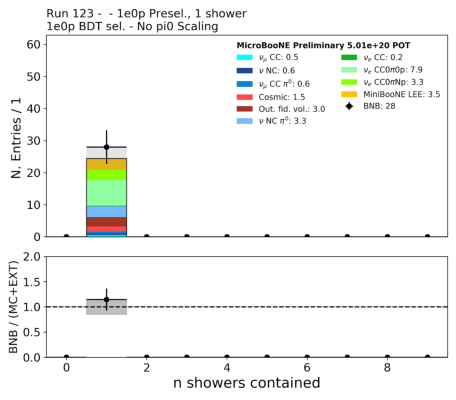
\includegraphics[width=1.00\textwidth]{Fakedata/set1/zp_postsel_nshr.pdf}
    \caption{\label{fig:fakedata:set1:zp_postsel_nshr} Number of showers.}
    \end{subfigure}
\caption{\label{fig:fakedata:set1:zpsel} 1e0p BDT selection.}
\end{center}
\end{figure}

The muon neutrino and exclusive electron neutrino selections are then passed to SBNfit to perform a constraint of the systmeatic uncertainties through a joint fit of $\nu_{\mu}$ and $\nu_e$ channels, following which a LEE-signal sensitivity is extracted.  Full systematic uncertainties are included: flux, genie, and detector.  %In all of the constraint plots the red line corresponds to the MC without any LEE hypothesis. 
Fig. ~\ref{fig:fakedata:set1:numu_const} shows the muon neutrino selection before and after the constraint. After the constraint is performed the muon neutrino prediction collapses to the observed data as a result of the $\chi^2$-based constraint.
Fig. ~\ref{fig:fakedata:set1:np_const} shows the 1eNp selection before and after the constraint, and Fig. ~\ref{fig:fakedata:set1:np_const} the 1e0p selection.  In both selections the excess at low energy increases after the constraint is performed.    
\begin{figure}[H] 
\begin{center}
    \begin{subfigure}[b]{0.45\textwidth}
    \centering
    %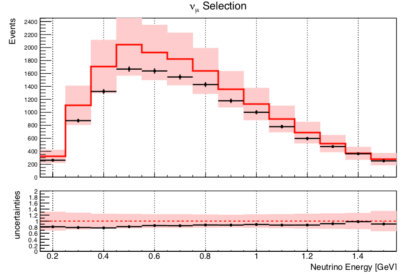
\includegraphics[width=1.00\textwidth]{Fakedata/set1/numu_before_constrain.pdf}
    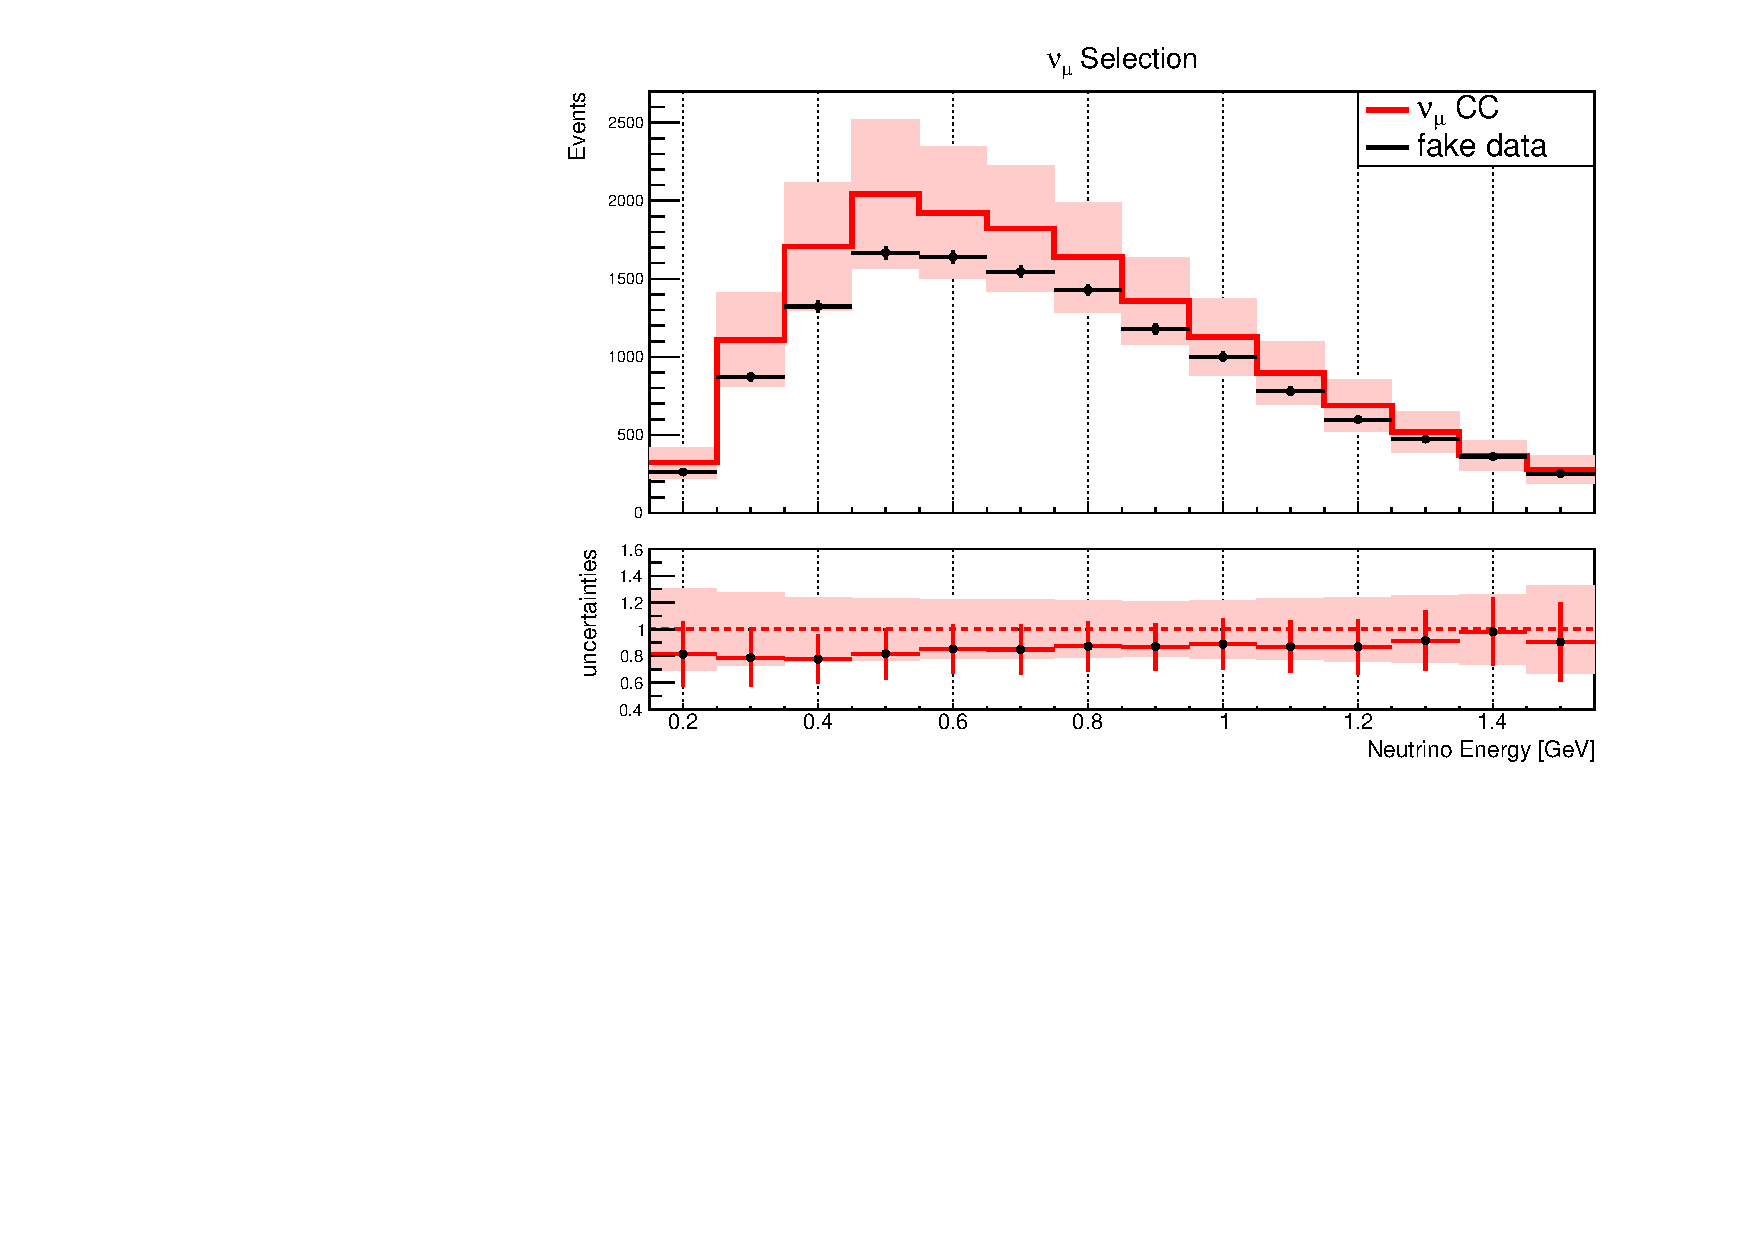
\includegraphics[width=1.00\textwidth]{Fakedata/set1/nue_numu_reco_e_H1_mc_fakedata_set1_numu_before_data_constraint.pdf}
    \caption{\label{fig:fakedata:set1:numu_before_constrain} Before constraint.}
    \end{subfigure}
    \begin{subfigure}[b]{0.45\textwidth}
    \centering
    %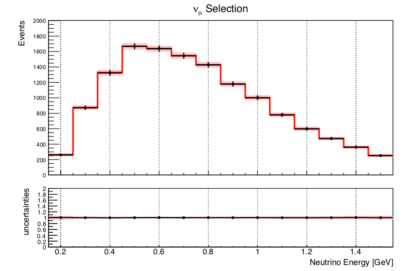
\includegraphics[width=1.00\textwidth]{Fakedata/set1/numu_after_constrain.pdf}
    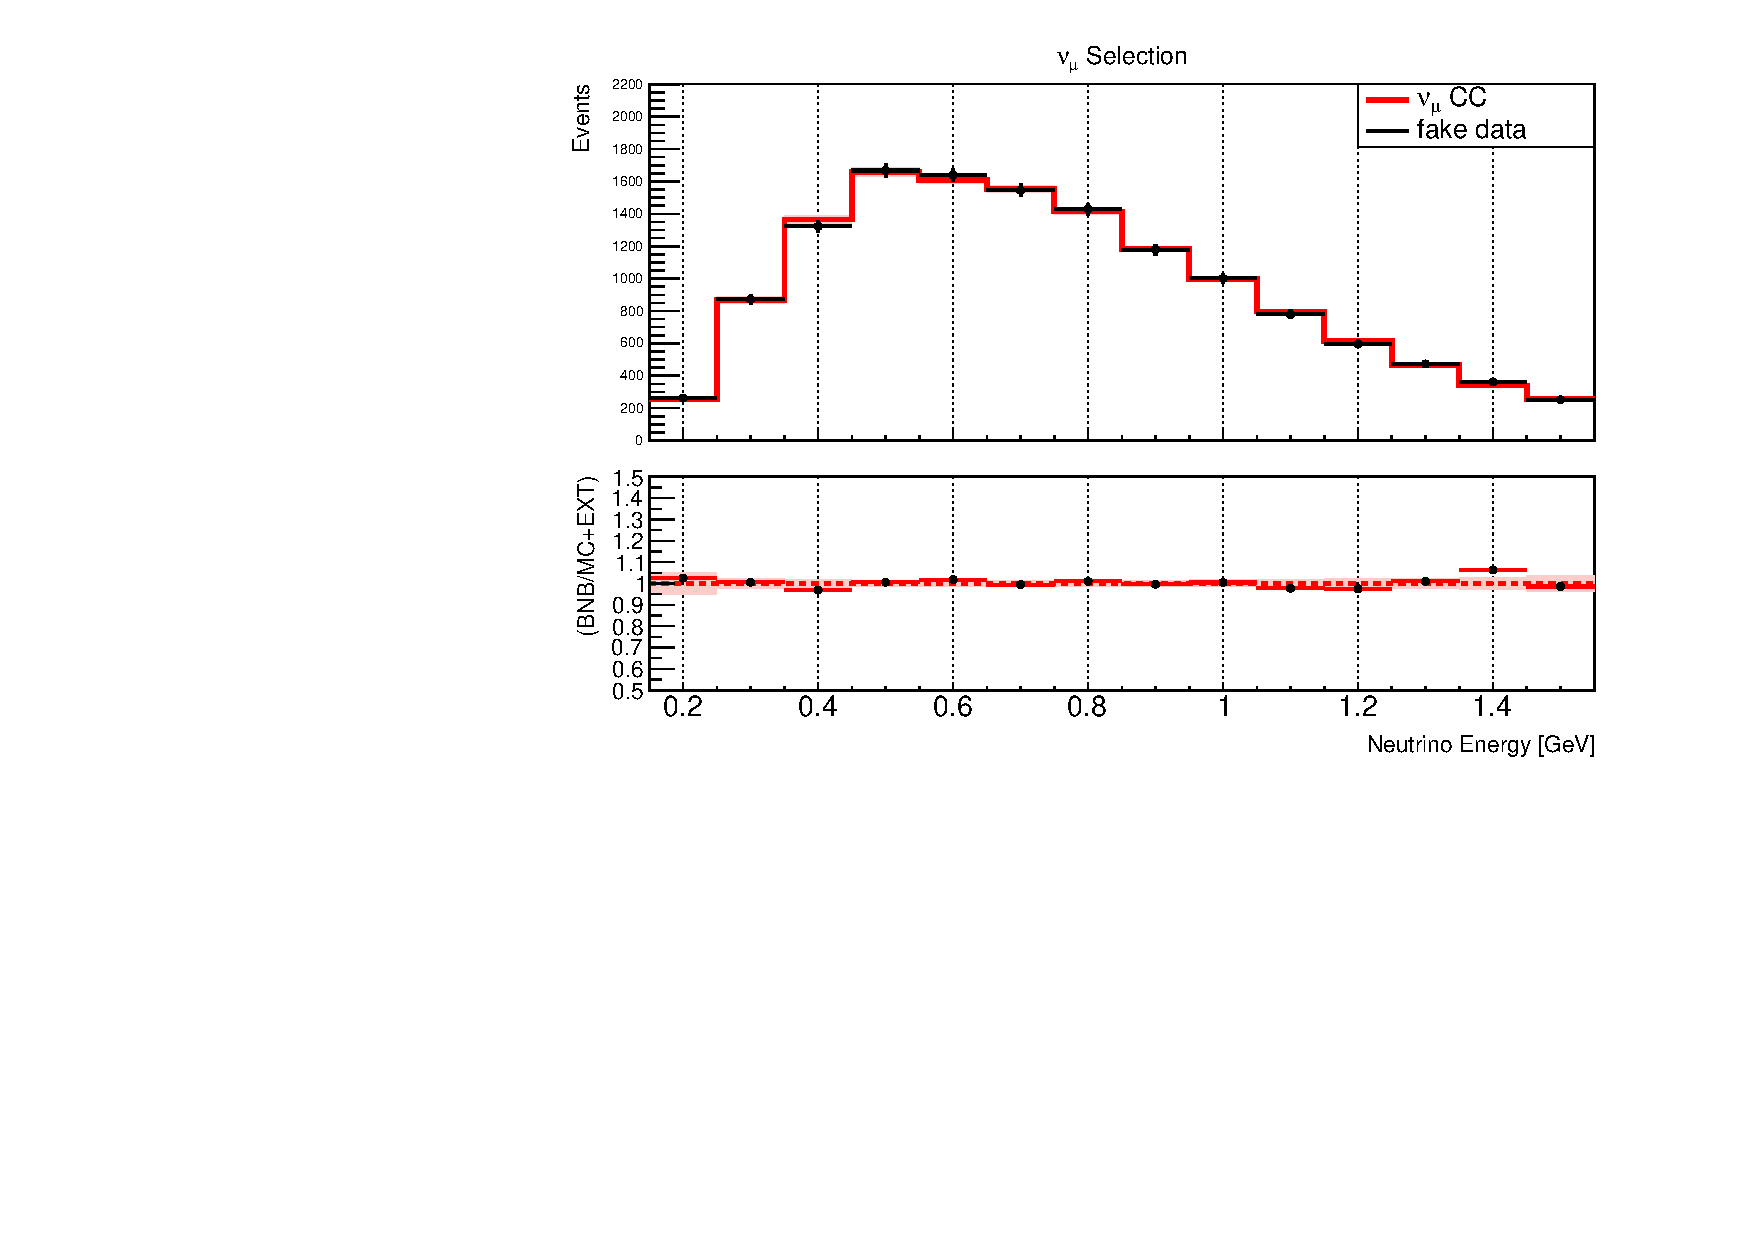
\includegraphics[width=1.00\textwidth]{Fakedata/set1/nue_numu_reco_e_H1_mc_fakedata_set1_scaled_numu.pdf}
    \caption{\label{fig:fakedata:set1:numu_after_constrain} After constraint.}
    \end{subfigure}
\caption{\label{fig:fakedata:set1:numu_const} Muon neutrino selection.}
\end{center}
\end{figure}

\begin{figure}[H] 
\begin{center}
    \begin{subfigure}[b]{0.45\textwidth}
    \centering
    %\includegraphics[width=1.00\textwidth]{Fakedata/set1/np_before_constrain.pdf}
    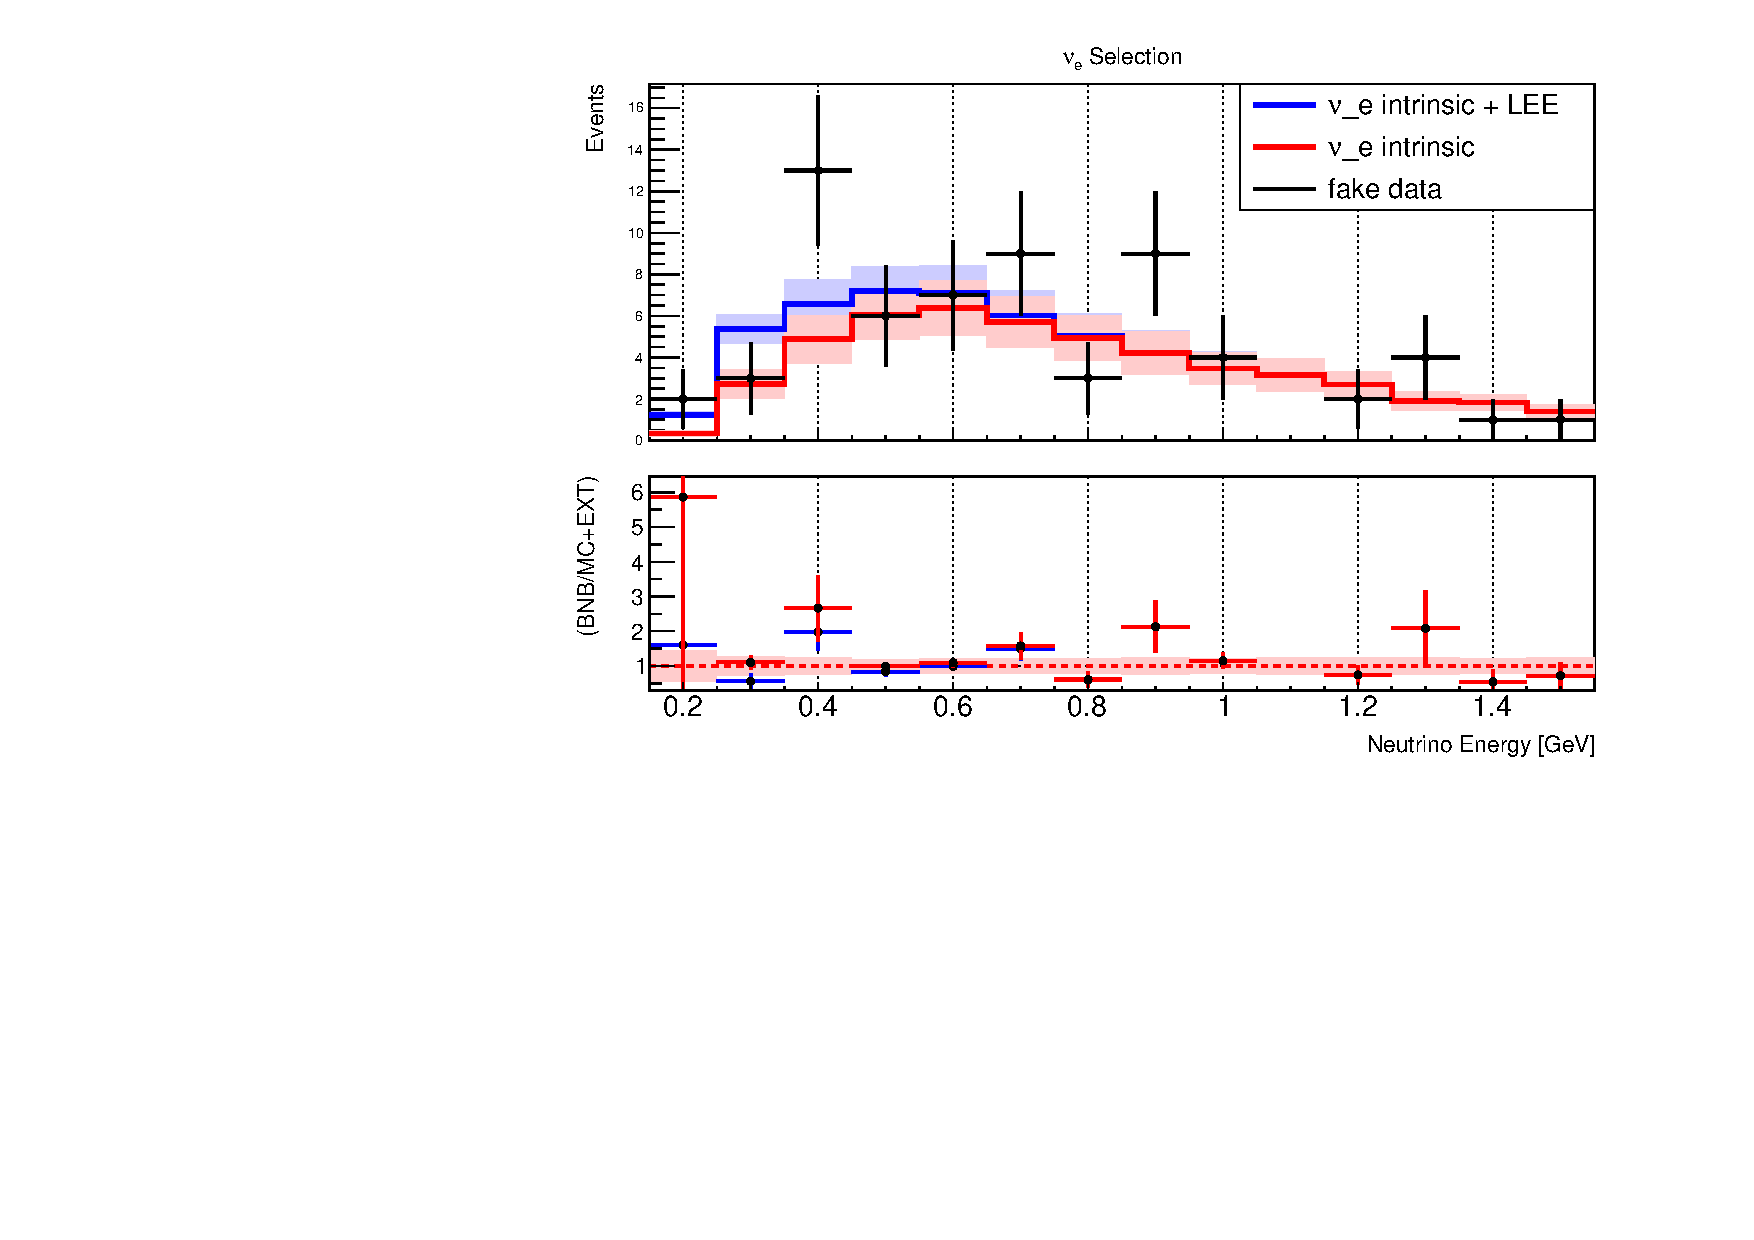
\includegraphics[width=1.00\textwidth]{Fakedata/set1/nue_numu_reco_e_H1_mc_fakedata_set1_nue_before_data_constraint.pdf}
    \caption{\label{fig:fakedata:set1:np_before_constrain} Before constraint.}
    \end{subfigure}
    \begin{subfigure}[b]{0.45\textwidth}
    \centering
    %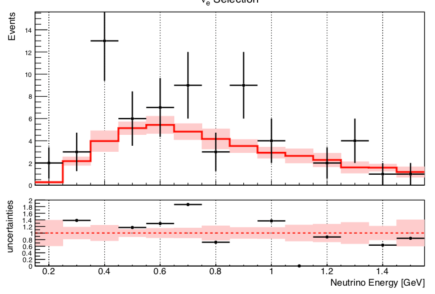
\includegraphics[width=1.00\textwidth]{Fakedata/set1/np_after_constrain.pdf}
    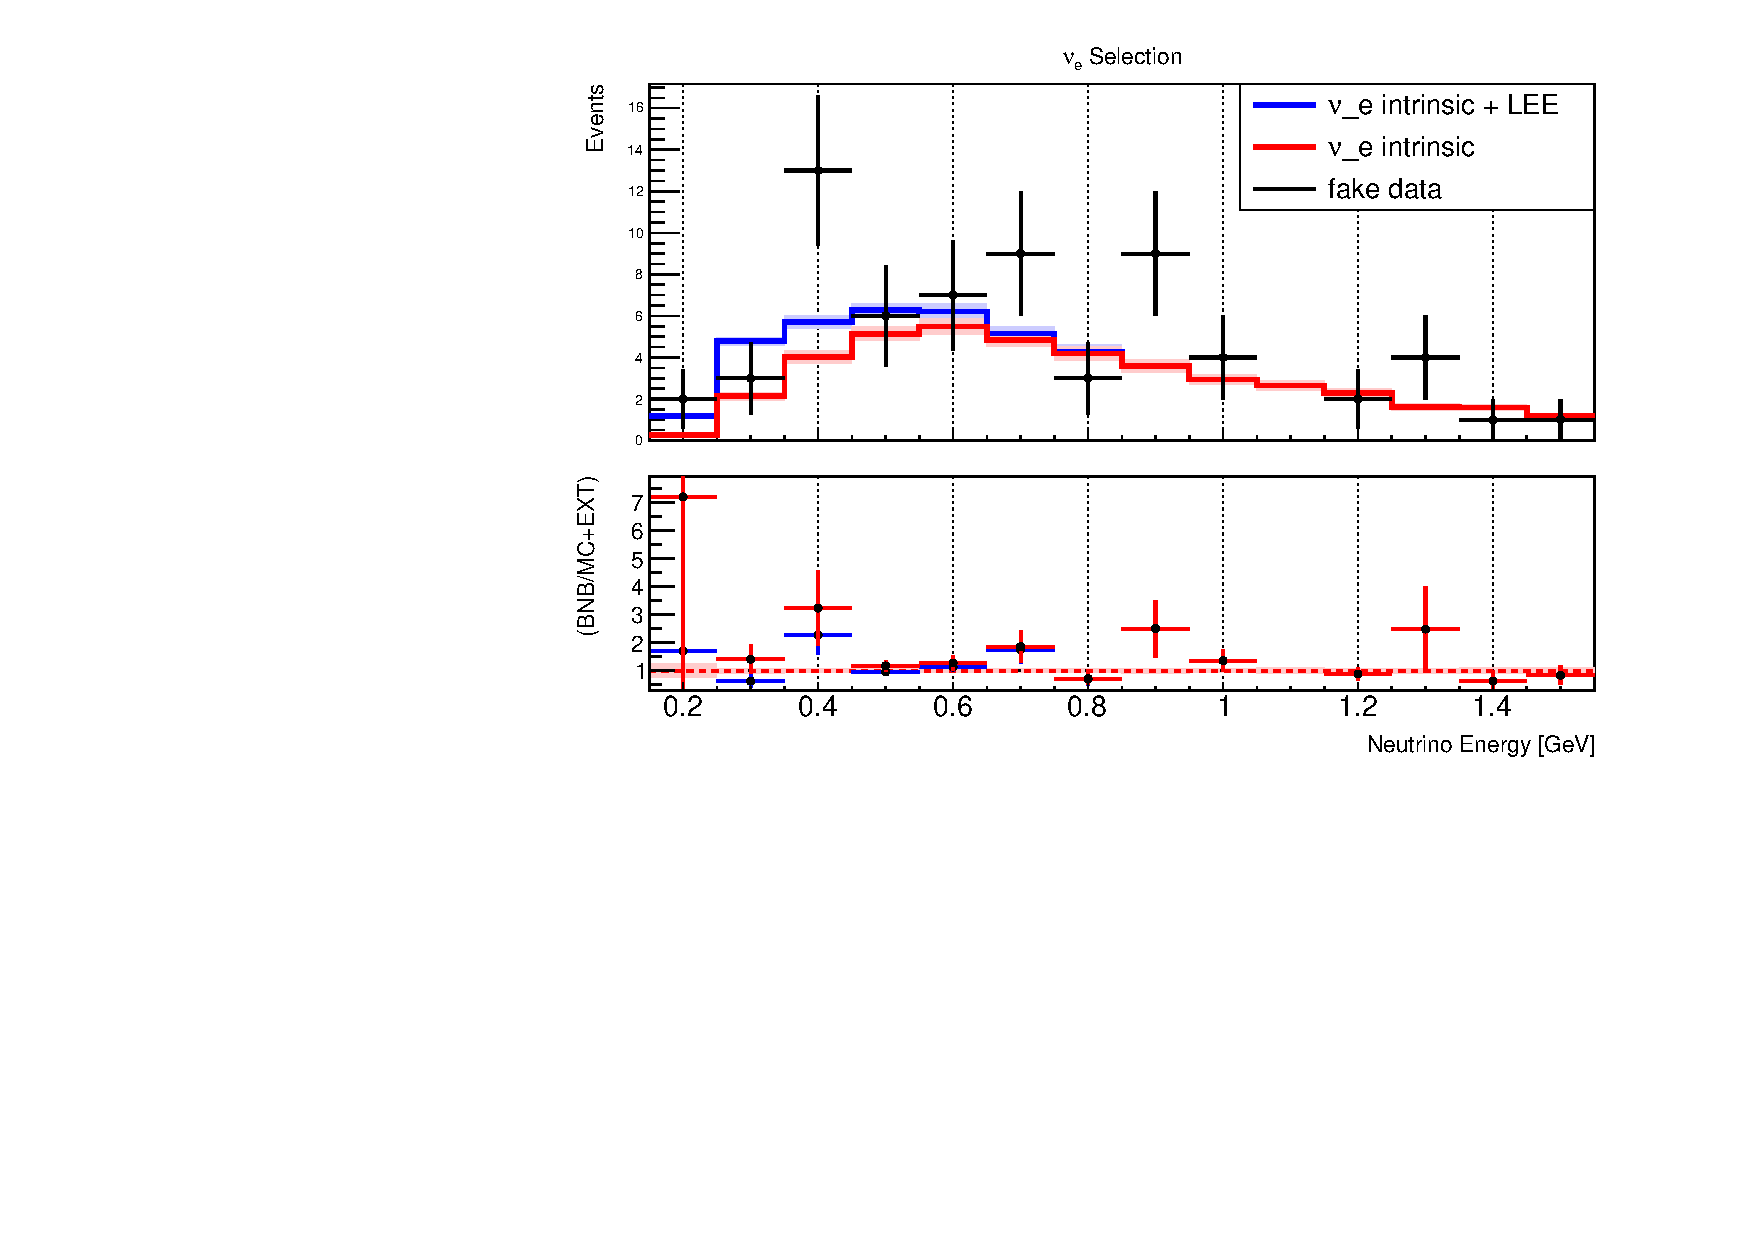
\includegraphics[width=1.00\textwidth]{Fakedata/set1/nue_numu_reco_e_H1_mc_fakedata_set1_univ_overlay_nue.pdf}
    \caption{\label{fig:fakedata:set1:np_after_constrain} After constraint.}
    \end{subfigure}
\caption{\label{fig:fakedata:set1:np_const} 1eNp selection.}
\end{center}
\end{figure}

\begin{figure}[H] 
\begin{center}
    \begin{subfigure}[b]{0.45\textwidth}
    \centering
    %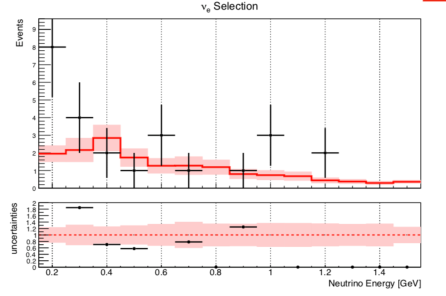
\includegraphics[width=1.00\textwidth]{Fakedata/set1/zp_before_constrain.pdf}
    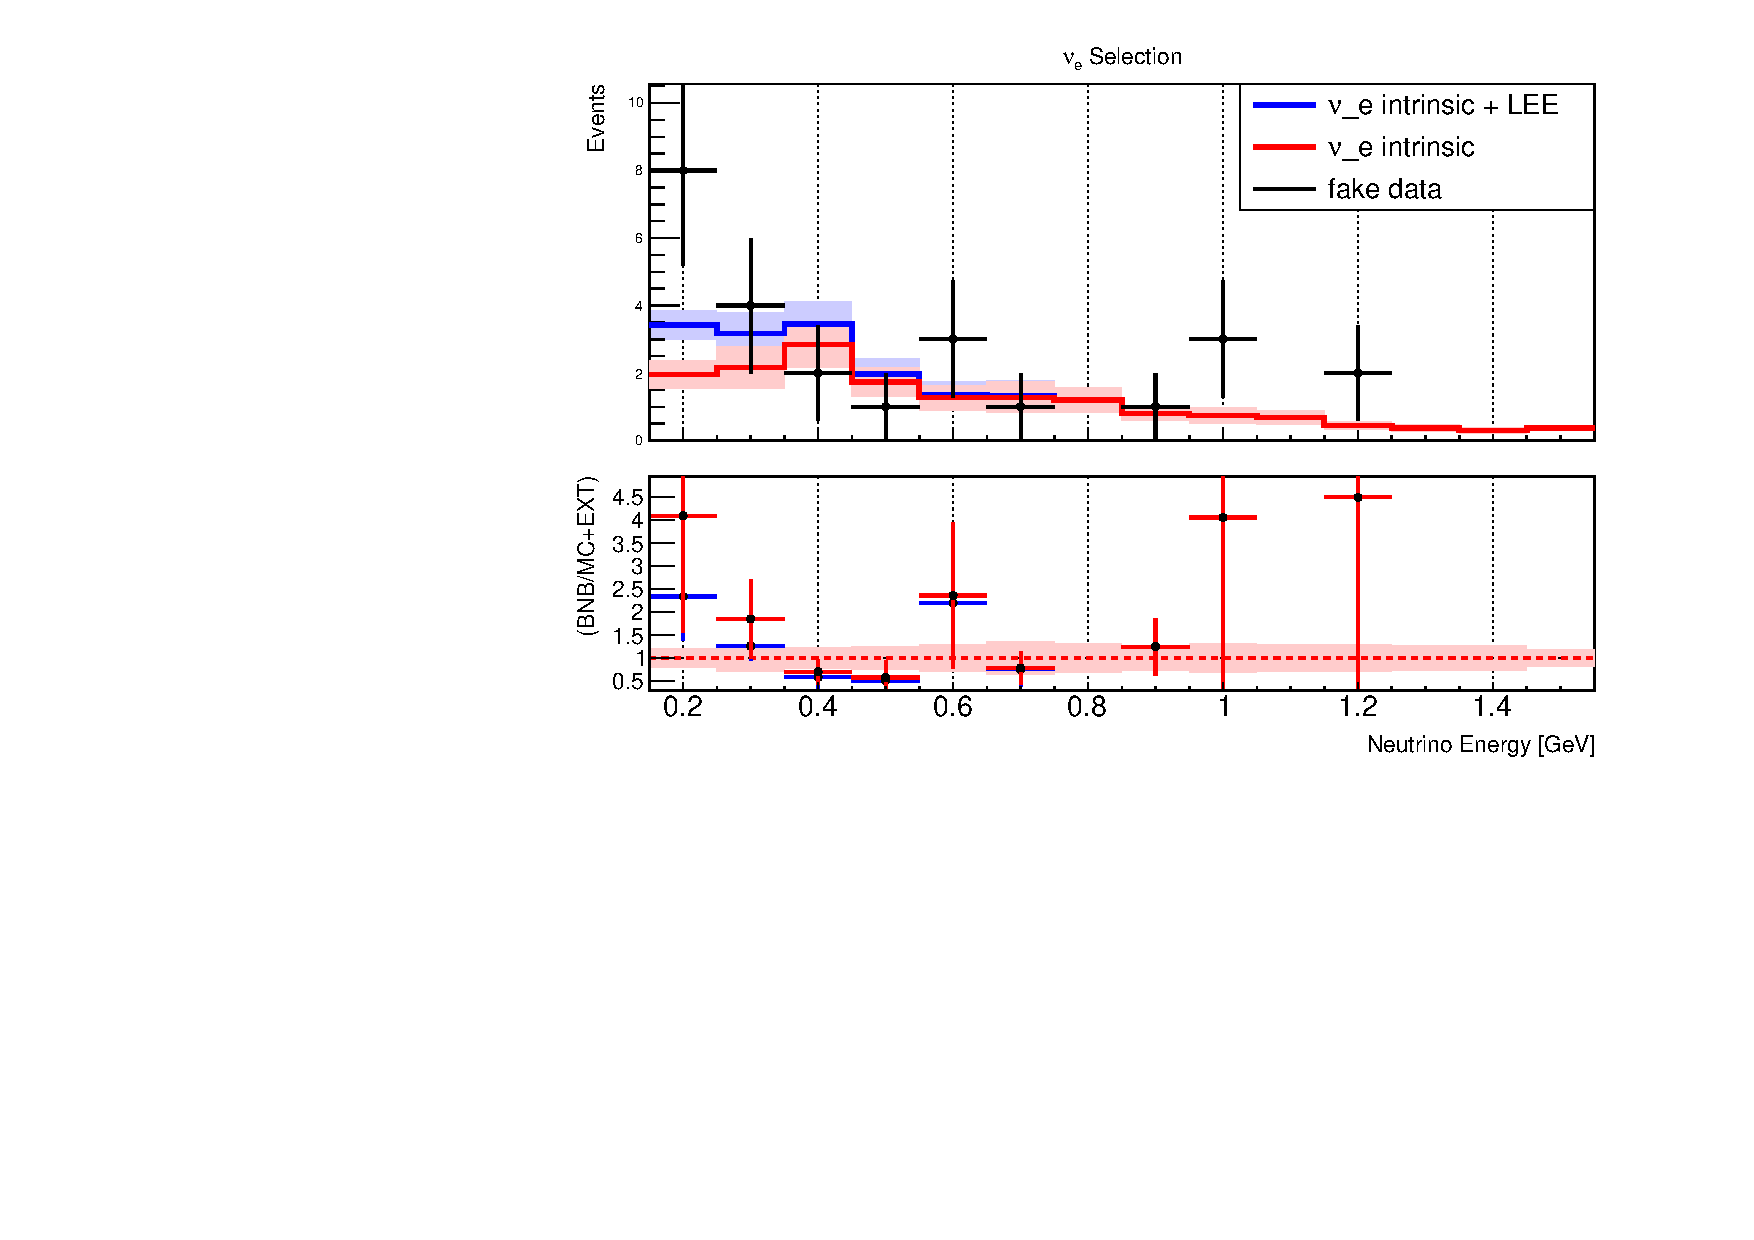
\includegraphics[width=1.00\textwidth]{Fakedata/set1/1e0p_numu_reco_e_H1_mc_fakedata_set1_nue_before_data_constraint.pdf}
    \caption{\label{fig:fakedata:set1:zp_before_constrain} Before constraint.}
    \end{subfigure}
    \begin{subfigure}[b]{0.45\textwidth}
    \centering
    %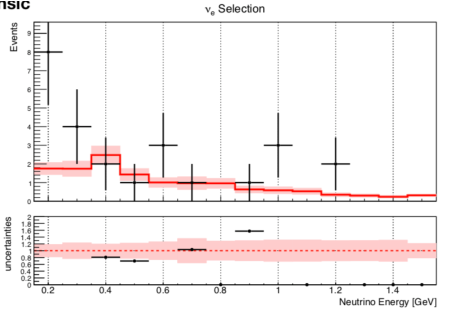
\includegraphics[width=1.00\textwidth]{Fakedata/set1/zp_after_constrain.pdf}
    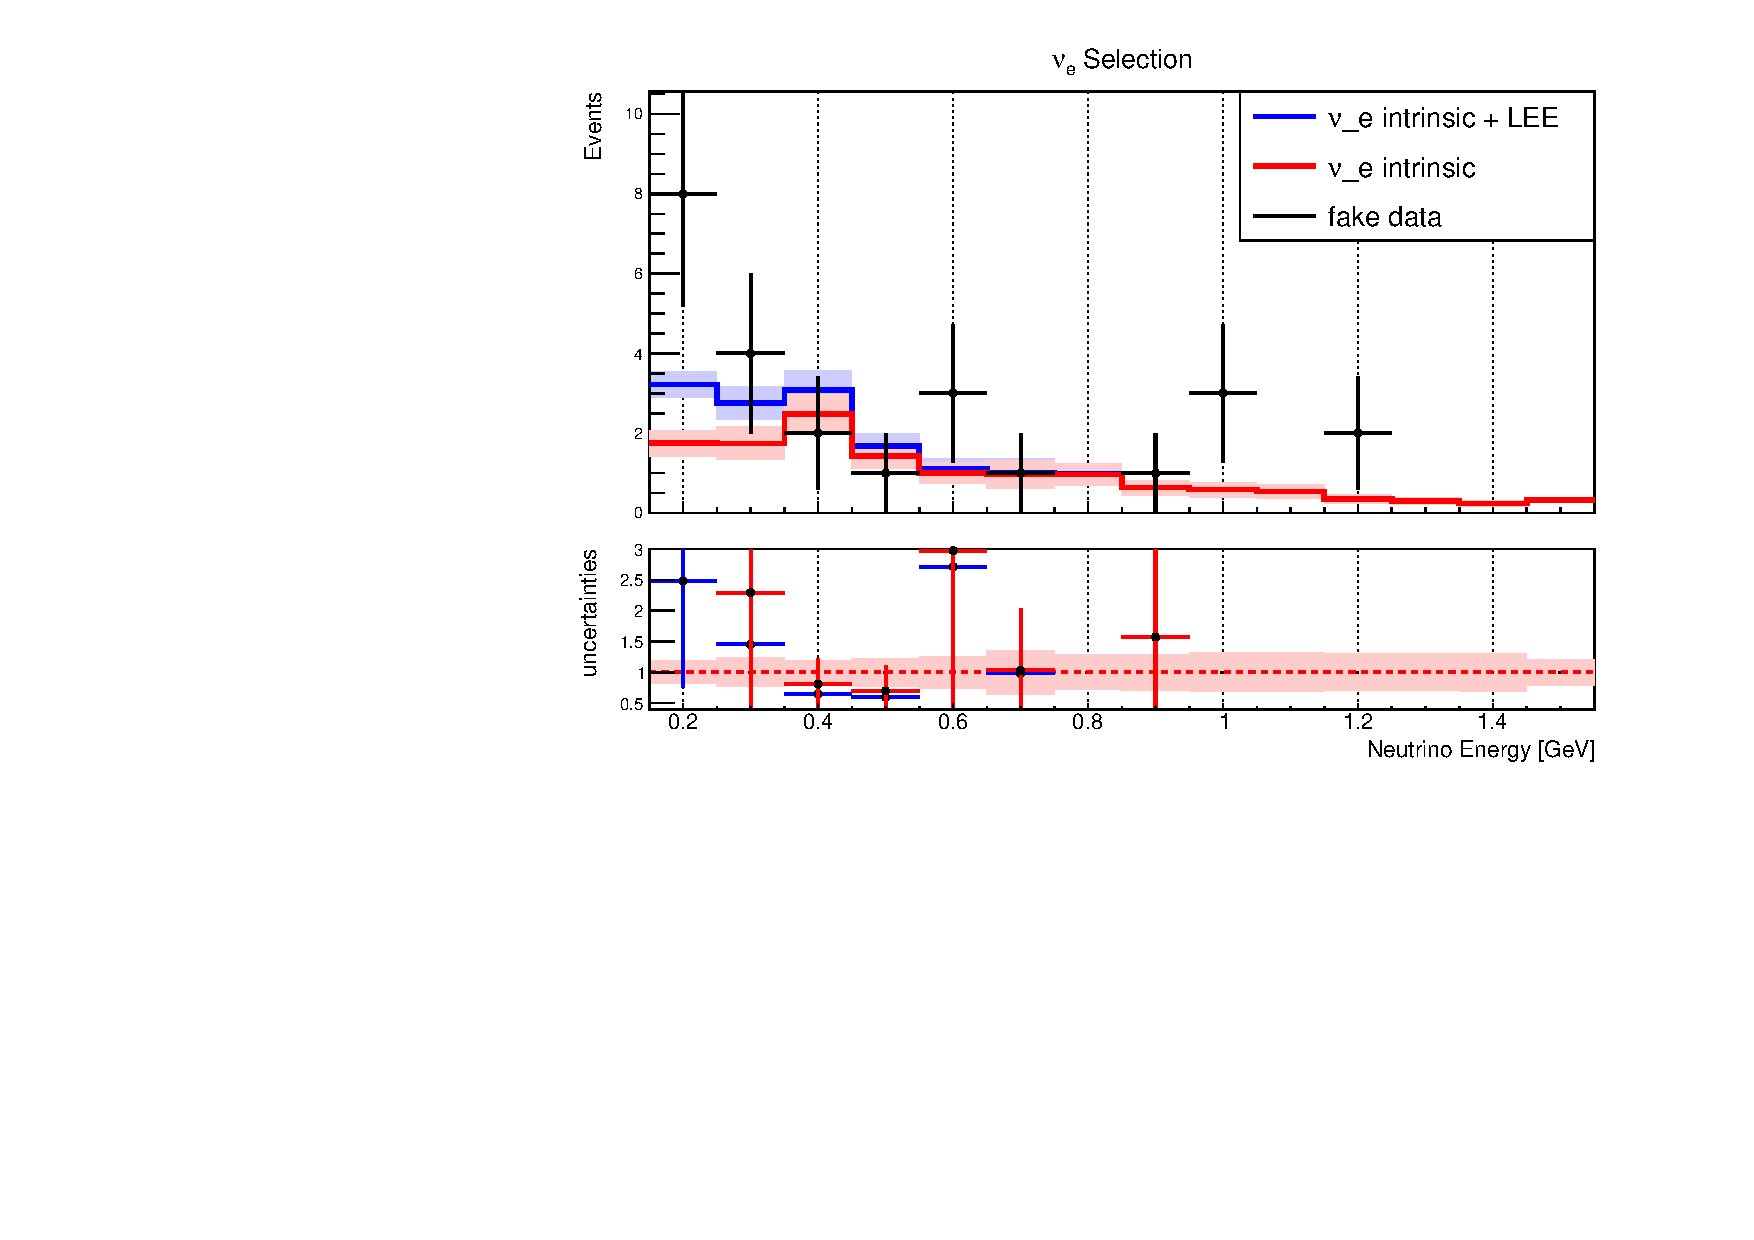
\includegraphics[width=1.00\textwidth]{Fakedata/set1/1e0p_numu_reco_e_H1_mc_fakedata_set1_univ_overlay_nue.pdf}
    \caption{\label{fig:fakedata:set1:zp_after_constrain} After constraint.}
    \end{subfigure}
\caption{\label{fig:fakedata:set1:zp_const} 1e0p selection.}
\end{center}
\end{figure}

The sensitivity can then be calculated using the joint fit procedure within SBNFit. The $\Delta \chi^{2}$ for the LEE and standard model hypotheses are shown in Fig.~\ref{fig:fakedata:set1:sens}.  $\Delta \chi^{2}$ is defined as $\chi^{2}_{{\rm fakedata}, H_{0}}-\chi^{2}_{{\rm fakedata}, H_{1}}$. The sensitivity to rule out the standard model if the LEE is true for fake data set 1 is 3.4 sigma.  The median sensitivity is 2.2 sigma. This means that the fit prefers the unfolded LEE model over the standard model for fake dataset 1.

\begin{figure}[H]
\begin{center}
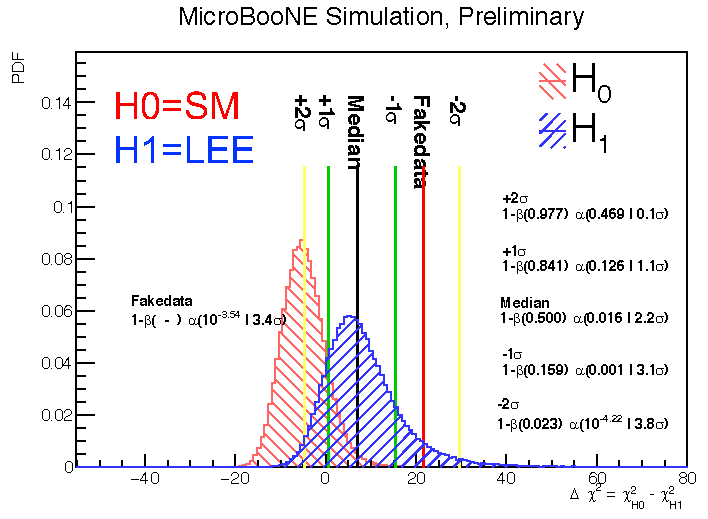
\includegraphics[width=0.75\textwidth]{Fakedata/set1/sens.pdf}
\caption{\label{fig:fakedata:set1:sens} $\Delta \chi^{2}$ for fake data set relative to standard model and LEE hypotheses. The $\chi^{2}$ for the $H_0$ hypothesis is $67.2$, the $\chi^{2}$ for the $H_1$ hypothesis is $46.7$, and the resulting $\Delta \chi^{2}$ is $20.5$ }
\end{center}
\end{figure}

%%%%%%%%%%%%%%%%%%%%%%%%%%%%%%%%%

\subsection{Set 2}

The first selections studied are those rich in $\pi^{0}$s. Fig~\ref{fig:fakedata:set2:pi0} shows the reconstructed $\pi^{0}$ mass for the $\pi^{0}$ selection. Good data-MC agreement is observed, as well as good energy scale resolution in the reconstructed $\pi^{0}$ mass. 
\begin{figure}[H]
\begin{center}
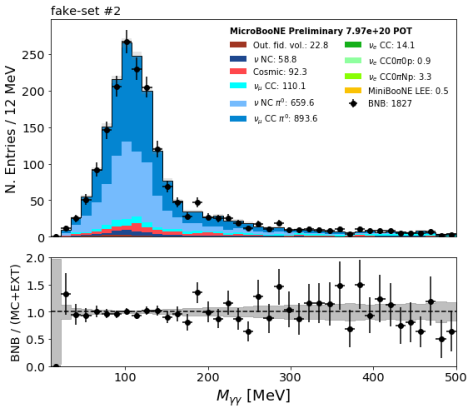
\includegraphics[width=0.45\textwidth]{Fakedata/set2/pi0.pdf}
\caption{\label{fig:fakedata:set2:pi0} $\pi^{0}$ selection.}
\end{center}
\end{figure}

Fig~\ref{fig:fakedata:set2:2shr} shows the 2+ shower side band for the 1eNp and 1e0p selections. There is good agreement in the 2+ shower side band in the 1e0p and 1eNp selections.  

\begin{figure}[H] 
\begin{center}
    \begin{subfigure}[b]{0.45\textwidth}
    \centering
    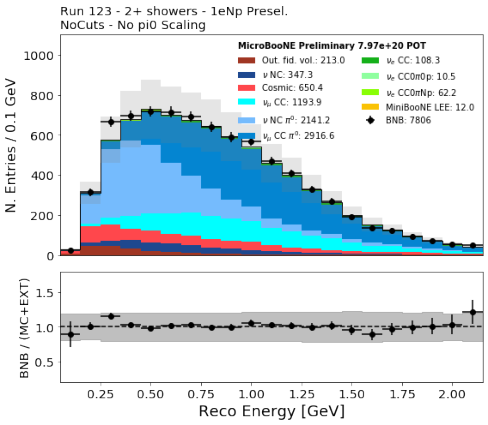
\includegraphics[width=1.00\textwidth]{Fakedata/set2/np_2shr.pdf}
    \caption{\label{fig:fakedata:set2:2shrnp} 1eNp at pre-selection}
    \end{subfigure}
    \begin{subfigure}[b]{0.45\textwidth}
    \centering
    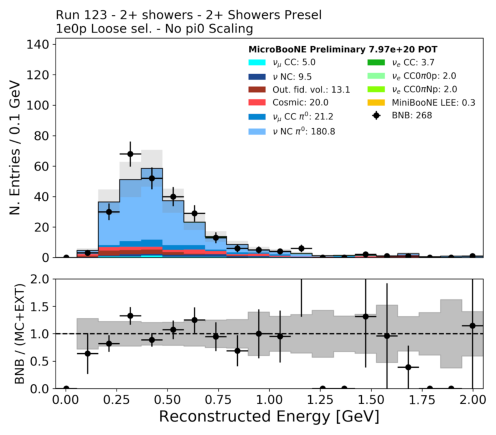
\includegraphics[width=1.00\textwidth]{Fakedata/set2/zp_2shr.pdf}
    \caption{\label{fig:fakedata:set2:2shr0p} 1e0p after loose selection}
    \end{subfigure}
\caption{\label{fig:fakedata:set2:2shr} 2+ shower side bands.}
\end{center}
\end{figure}

The inclusive electron neutrino selection is sensitive to the electron neutrino content in the beam and can also be used to measure data-MC agreement.  Fig~\ref{fig:fakedata:set2:inc_presel} shows the shower dE/dx of the inclusive selection at pre-selection.  The distribution agrees within errors.   

\begin{figure}[H]
\begin{center}
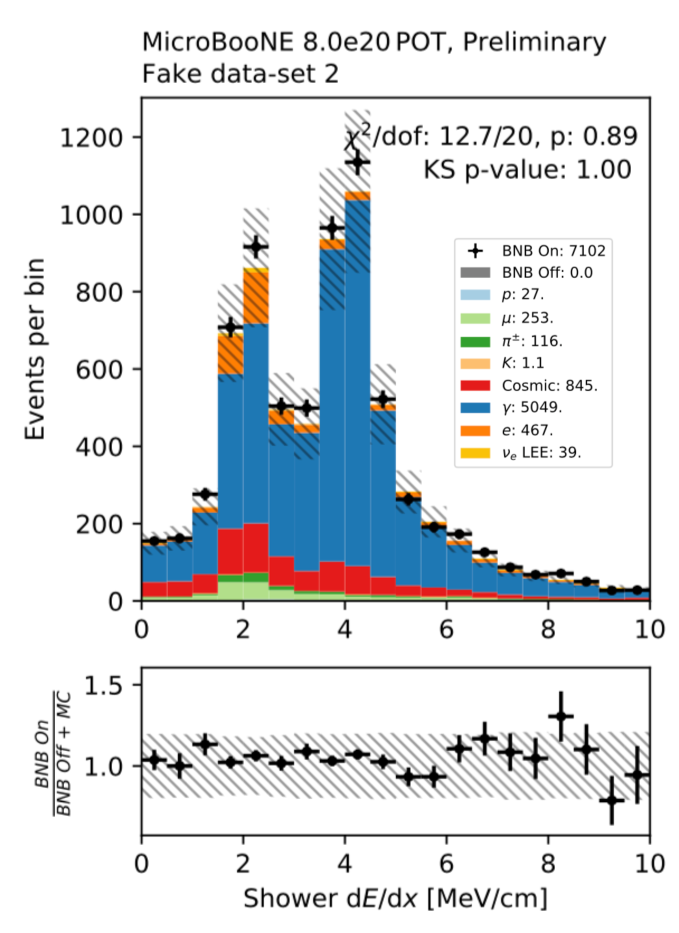
\includegraphics[width=0.45\textwidth]{Fakedata/set2/inc_presel.pdf}
\caption{\label{fig:fakedata:set2:inc_presel} dE/dx of inclusive selection at pre-selection.}
\end{center}
\end{figure}

Fig~\ref{fig:fakedata:set2:inc_postsel} shows the final inclusive selection in electron shower energy, shower theta and track multiplicity.  After selection these distributions agree within errors.

\begin{figure}[H]
\begin{center}
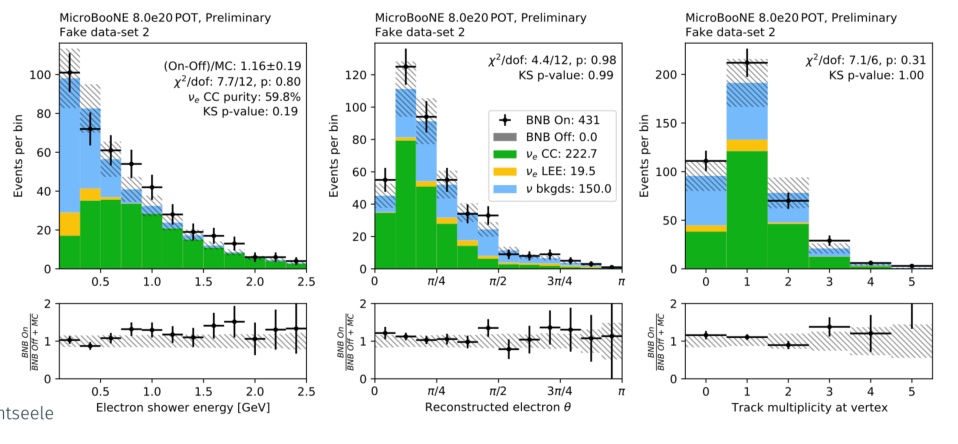
\includegraphics[width=0.9\textwidth]{Fakedata/set2/incl_postsel.pdf}
\caption{\label{fig:fakedata:set2:inc_postsel} Inclusive selection of electron neutrinos. From left to right: electron shower energy, shower theta, track multiplicity.}
\end{center}
\end{figure}

The muon neutrino selection data-MC agreement was also studied in the fake data.  Only the run 3 fake data is used because the CRT is used in the selection. Comparisons where runs 1 and 3 are combined show similar effects to the ones observed here. 
Fig~\ref{fig:fakedata:set2:numu} shows the muon neutrino selection in lepton angle, energy, and total number of tracks. Overall high normalization is observed in most variables in the muon neutrino selection.  This variation is within the systematic uncertainty so that the covariance matrix fit can account for the differences.

\begin{figure}[H] 
\begin{center}
    \begin{subfigure}[b]{0.3\textwidth}
    \centering
    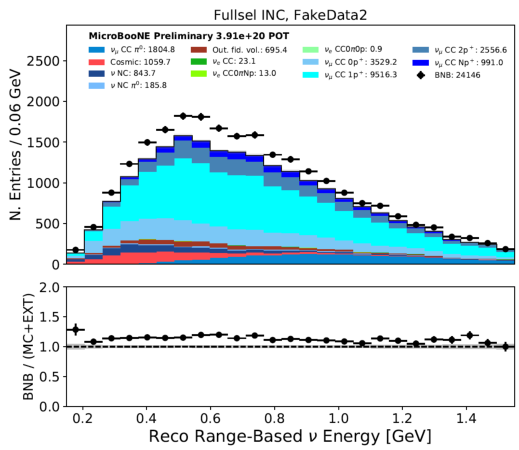
\includegraphics[width=1.00\textwidth]{Fakedata/set2/numu_energy.pdf}
    \caption{\label{fig:fakedata:set2:numu_energy} Energy.}
    \end{subfigure}
    \begin{subfigure}[b]{0.3\textwidth}
    \centering
    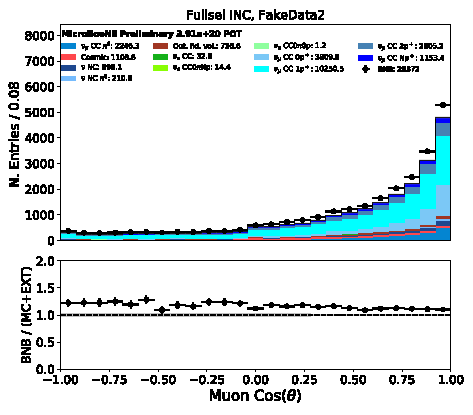
\includegraphics[width=1.00\textwidth]{Fakedata/set2/numu_costheta.pdf}
    \caption{\label{fig:fakedata:set2:numu_costheta} cos($\theta$)}
    \end{subfigure}
    \begin{subfigure}[b]{0.3\textwidth}
    \centering
    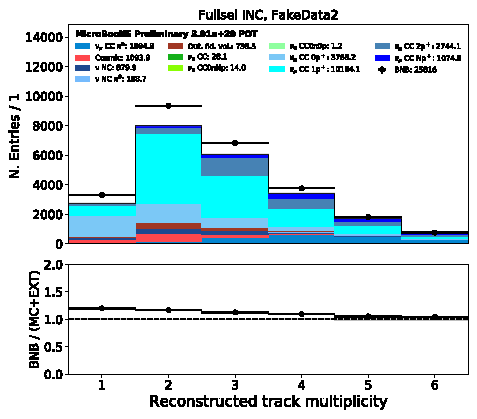
\includegraphics[width=1.00\textwidth]{Fakedata/set2/numu_ntracks.pdf}
    \caption{\label{fig:fakedata:set2:numu_ntracks} Number of tracks}
    \end{subfigure}
\caption{\label{fig:fakedata:set2:numu} Muon neutrino selection. Systematic uncertainties are not plotted, but are included in the constraint.}
\end{center}
\end{figure}

The exclusive electron neutrino selections were also performed on the fake data. Fig~\ref{fig:fakedata:set2:presel} shows the reconstructed energy of events passing the 1eNp and 1e0p pre-selections.  Good agreement is observed in both cases.

\begin{figure}[H] 
\begin{center}
    \begin{subfigure}[b]{0.45\textwidth}
    \centering
    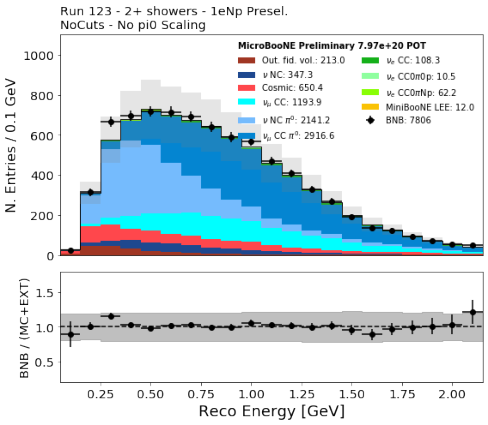
\includegraphics[width=1.00\textwidth]{Fakedata/set2/np_2shr.pdf}
    \caption{\label{fig:fakedata:set2:Np_presel_recoe} 1eNp at pre-selection}
    \end{subfigure}
    \begin{subfigure}[b]{0.45\textwidth}
    \centering
    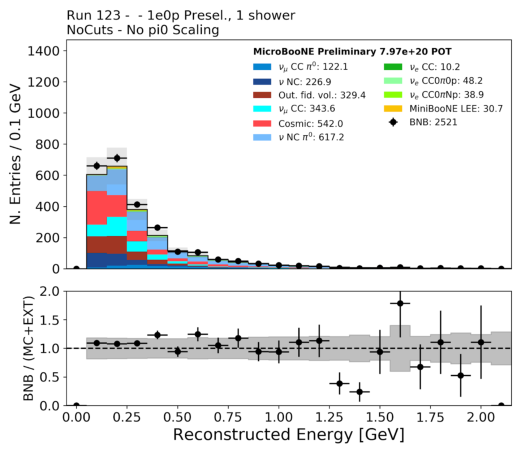
\includegraphics[width=1.00\textwidth]{Fakedata/set2/zp_presel_recoe.pdf}
    \caption{\label{fig:fakedata:set2:2shr0p} 1e0p after pre-selection}
    \end{subfigure}
\caption{\label{fig:fakedata:set2:presel} Exclusive electron neutrino selections at pre-selection stage.}
\end{center}
\end{figure}

Fig~\ref{fig:fakedata:set2:npsel} shows various distributions after the 1eNp BDT selection.  An excess is observed at medium reconstructed neutrino energy. There is also an excess in one track events relative the prediction.

\begin{figure}[H] 
\begin{center}
    \begin{subfigure}[b]{0.45\textwidth}
    \centering
    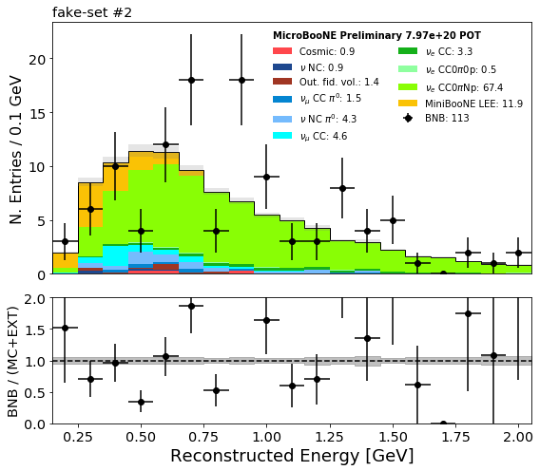
\includegraphics[width=1.00\textwidth]{Fakedata/set2/Np_postsel_recoe.pdf}
    \caption{\label{fig:fakedata:set2:Np_postsel_recoe} Reconstructed energy.}
    \end{subfigure}
    \begin{subfigure}[b]{0.45\textwidth}
    \centering
    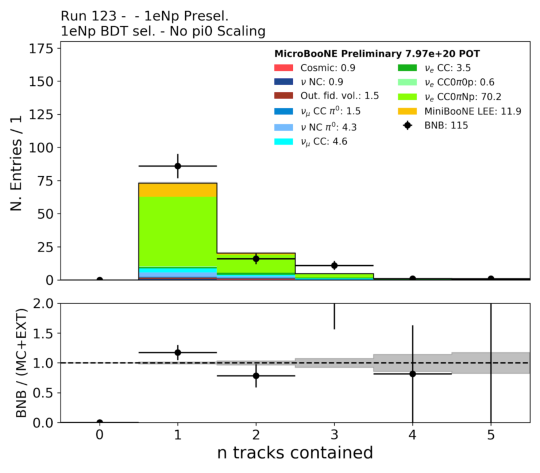
\includegraphics[width=1.00\textwidth]{Fakedata/set2/Np_postsel_ntracks.pdf}
    \caption{\label{fig:fakedata:set2:Np_postsel_ntracks} Number of tracks.}
    \end{subfigure}
\caption{\label{fig:fakedata:set2:npsel} 1eNp BDT selection.}
\end{center}
\end{figure}

Fig~\ref{fig:fakedata:set2:zpsel} shows the 1e0p selection after BDT selection.  There is agreement at low energy after the BDT selection and in overall normalization. An excess is observed at high BDT response.

\begin{figure}[H] 
\begin{center}
    \begin{subfigure}[b]{0.3\textwidth}
    \centering
    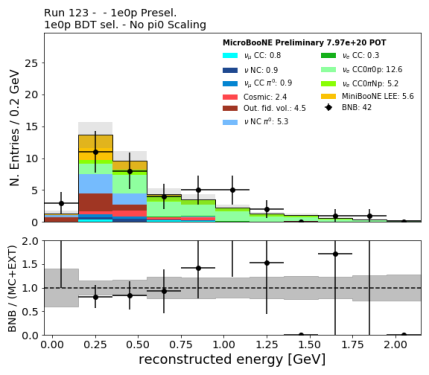
\includegraphics[width=1.00\textwidth]{Fakedata/set2/zp_postsel_recoe.pdf}
    \caption{\label{fig:fakedata:set2:zp_postsel_recoe} Reconstructed energy.}
    \end{subfigure}
    \begin{subfigure}[b]{0.3\textwidth}
    \centering
    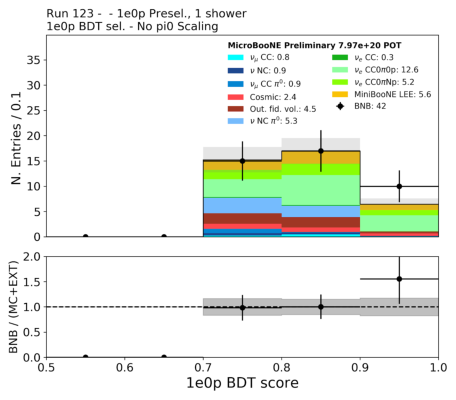
\includegraphics[width=1.00\textwidth]{Fakedata/set2/zp_postsel_bdt.pdf}
    \caption{\label{fig:fakedata:set2:zp_postsel_bdt} BDT response.}
    \end{subfigure}
    \begin{subfigure}[b]{0.3\textwidth}
    \centering
    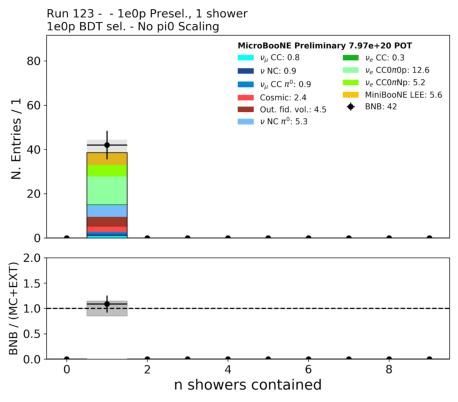
\includegraphics[width=1.00\textwidth]{Fakedata/set2/zp_postsel_nshr.pdf}
    \caption{\label{fig:fakedata:set2:zp_postsel_nshr} Number of showers.}
    \end{subfigure}
\caption{\label{fig:fakedata:set2:zpsel} 1e0p BDT selection.}
\end{center}
\end{figure}

The muon neutrino and exclusive electron neutrino selections are then passed to SBNfit to perform a constraint of the systematic uncertainties, and a fit to the sensitivity.  Full systematic uncertainties are included: flux, genie, geant re-interaction, and detector.  In all of the constraint plots the red line corresponds to the MC without any LEE hypothesis. Fig. ~\ref{fig:fakedata:set2:numu_const} shows the muon neutrino selection before and after the constraint. After the constraint is performed the muon neutrino data agrees well with the prediction.   
Fig. ~\ref{fig:fakedata:set2:np_const} shows the 1eNp selection before and after the constraint, and Fig. ~\ref{fig:fakedata:set2:np_const} the 1e0p selection.  In both selections the small data excess relative to prediction is  mitigated by the constraint.

\begin{figure}[H] 
\begin{center}
    \begin{subfigure}[b]{0.45\textwidth}
    \centering
    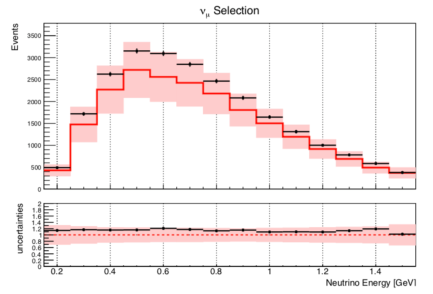
\includegraphics[width=1.00\textwidth]{Fakedata/set2/numu_before_constrain.pdf}
    \caption{\label{fig:fakedata:set2:numu_before_constrain} Before constraint.}
    \end{subfigure}
    \begin{subfigure}[b]{0.45\textwidth}
    \centering
    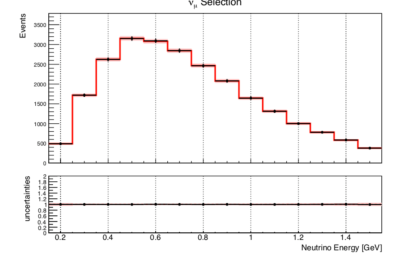
\includegraphics[width=1.00\textwidth]{Fakedata/set2/numu_after_constrain.pdf}
    \caption{\label{fig:fakedata:set2:numu_after_constrain} After constraint.}
    \end{subfigure}
\caption{\label{fig:fakedata:set2:numu_const} Muon neutrino selection.}
\end{center}
\end{figure}

\begin{figure}[H] 
\begin{center}
    \begin{subfigure}[b]{0.45\textwidth}
    \centering
    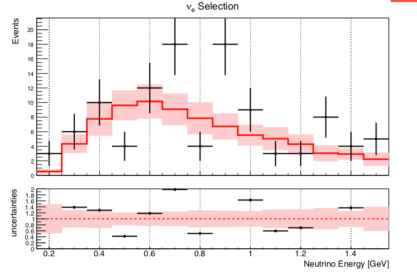
\includegraphics[width=1.00\textwidth]{Fakedata/set2/np_before_constrain.pdf}
    \caption{\label{fig:fakedata:set2:np_before_constrain} Before constraint.}
    \end{subfigure}
    \begin{subfigure}[b]{0.45\textwidth}
    \centering
    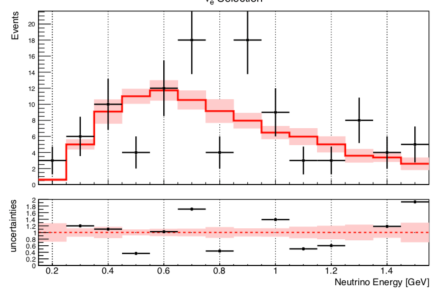
\includegraphics[width=1.00\textwidth]{Fakedata/set2/np_after_constrain.pdf}
    \caption{\label{fig:fakedata:set2:np_after_constrain} After constraint.}
    \end{subfigure}
\caption{\label{fig:fakedata:set2:np_const} 1eNp selection.}
\end{center}
\end{figure}

\begin{figure}[H] 
\begin{center}
    \begin{subfigure}[b]{0.45\textwidth}
    \centering
    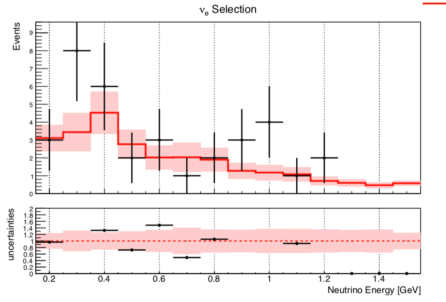
\includegraphics[width=1.00\textwidth]{Fakedata/set2/zp_before_constrain.pdf}
    \caption{\label{fig:fakedata:set2:zp_before_constrain} Before constraint.}
    \end{subfigure}
    \begin{subfigure}[b]{0.45\textwidth}
    \centering
    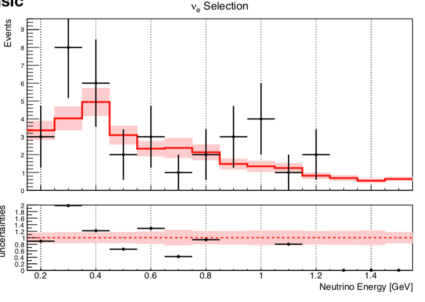
\includegraphics[width=1.00\textwidth]{Fakedata/set2/zp_after_constrain.pdf}
    \caption{\label{fig:fakedata:set2:zp_after_constrain} After constraint.}
    \end{subfigure}
\caption{\label{fig:fakedata:set2:zp_const} 1e0p selection.}
\end{center}
\end{figure}

The sensitivity can then be calculated using the joint fit procedure within SBNFit. The $\Delta \chi^{2}$ for the LEE and standard model hypotheses are shown in Fig.~\ref{fig:fakedata:set2:sens}.  $\Delta \chi^{2}$ is defined as $\chi^{2}_{fakedata, H_{0}}-\chi^{2}_{fakedata, H_{1}}$. The sensitivity to rule out the standard model if the LEE is true for fake data set 2 is 1.9 sigma.  The median sensitivity is 2.6 sigma. This result is inconclusive.

\begin{figure}[H]
\begin{center}
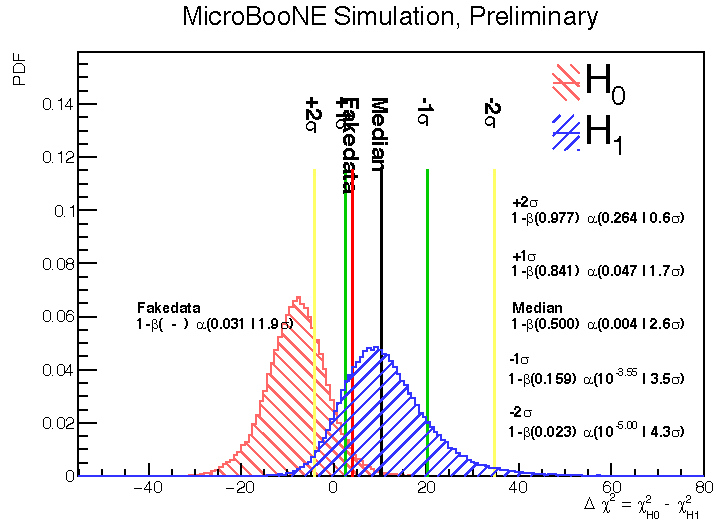
\includegraphics[width=0.75\textwidth]{Fakedata/set2/sens.pdf}
\caption{\label{fig:fakedata:set2:sens} $\Delta \chi^{2}$ for fake data set relative to standard model and LEE hypotheses. H0 is the standard model and H1 is the unfolded LEE model.}
\end{center}
\end{figure}

%%%%%%%%%%%%%%%%%%%%%%%%%%%

\subsection{Set 3}

The first selections studied are those rich in $\pi^{0}$s. Fig~\ref{fig:fakedata:set3:pi0} shows the reconstructed $\pi^{0}$ mass for the $\pi^{0}$ selection. Good data-MC agreement is observed, as well as good energy scale resolution in the reconstructed $\pi^{0}$ mass. 
\begin{figure}[H]
\begin{center}
\includegraphics[width=0.45\textwidth]{Fakedata/set3/pi0.pdf}
\caption{\label{fig:fakedata:set3:pi0} $\pi^{0}$ selection.}
\end{center}
\end{figure}

Fig~\ref{fig:fakedata:set3:2shr} shows the 2+ shower side band for the 1eNp and 1e0p selections. There is good agreement in the 2+ shower side band in the 1e0p selection.  There is an excess in the 2+ shower sideband with the Np selection relative to prediction observed at medium energy.  

\begin{figure}[H] 
\begin{center}
    \begin{subfigure}[b]{0.45\textwidth}
    \centering
    \includegraphics[width=1.00\textwidth]{Fakedata/set3/np_2shr.pdf}
    \caption{\label{fig:fakedata:set3:2shrnp} 1eNp at pre-selection}
    \end{subfigure}
    \begin{subfigure}[b]{0.45\textwidth}
    \centering
    \includegraphics[width=1.00\textwidth]{Fakedata/set3/zp_2shr.pdf}
    \caption{\label{fig:fakedata:set3:2shr0p} 1e0p after loose selection}
    \end{subfigure}
\caption{\label{fig:fakedata:set3:2shr} 2+ shower side bands.}
\end{center}
\end{figure}

The inclusive electron neutrino selection is sensitive to the electron neutrino content in the beam and can also be used to measure data-MC agreement.  Fig~\ref{fig:fakedata:set3:inc_presel} shows the shower dE/dx of the inclusive selection at pre-selection.  The distribution agrees within errors.   

\begin{figure}[H]
\begin{center}
\includegraphics[width=0.45\textwidth]{Fakedata/set3/inc_presel.pdf}
\caption{\label{fig:fakedata:set3:inc_presel} dE/dx of inclusive selection at pre-selection.}
\end{center}
\end{figure}

Fig~\ref{fig:fakedata:set3:inc_postsel} shows the final inclusive selection in electron shower energy, shower theta and track multiplicity.  After selection these distributions agree within errors.

\begin{figure}[H]
\begin{center}
\includegraphics[width=0.9\textwidth]{Fakedata/set3/incl_postsel.pdf}
\caption{\label{fig:fakedata:set3:inc_postsel} Inclusive selection of electron neutrinos. From left to right: electron shower energy, shower theta, track multiplicity.}
\end{center}
\end{figure}

The muon neutrino selection data-MC agreement was also studied in the fake data.  Only the run 3 fake data is used because the CRT is used in the selection. Comparisons where runs 1 and 3 are combined show similar effects to the ones observed here. 
Fig~\ref{fig:fakedata:set3:numu} shows the muon neutrino selection in lepton angle, energy, and total number of tracks. There are shape differences in many variables: more high-track events than predicted, and more events at medium-high energy.  These variations are within the systematic uncertainty so that the covariance matrix fit can account for the differences.

\begin{figure}[H] 
\begin{center}
    \begin{subfigure}[b]{0.3\textwidth}
    \centering
    \includegraphics[width=1.00\textwidth]{Fakedata/set3/numu_energy.pdf}
    \caption{\label{fig:fakedata:set3:numu_energy} Energy.}
    \end{subfigure}
    \begin{subfigure}[b]{0.3\textwidth}
    \centering
    \includegraphics[width=1.00\textwidth]{Fakedata/set3/numu_costheta.pdf}
    \caption{\label{fig:fakedata:set3:numu_costheta} cos($\theta$)}
    \end{subfigure}
    \begin{subfigure}[b]{0.3\textwidth}
    \centering
    \includegraphics[width=1.00\textwidth]{Fakedata/set3/numu_ntracks.pdf}
    \caption{\label{fig:fakedata:set3:numu_ntracks} Number of tracks}
    \end{subfigure}
\caption{\label{fig:fakedata:set3:numu} Muon neutrino selection. Systematic uncertainties are not plotted, but are included in the constraint.}
\end{center}
\end{figure}

The exclusive electron neutrino selections were also performed on the fake data. Fig~\ref{fig:fakedata:set3:presel} shows the reconstructed energy of events passing the 1eNp and 1e0p pre-selections.  Good agreement is observed in the 1e0p selection.  There is a shape difference in the reconstructed energy distribution in the Np events at pre-selection.

\begin{figure}[H] 
\begin{center}
    \begin{subfigure}[b]{0.45\textwidth}
    \centering
    \includegraphics[width=1.00\textwidth]{Fakedata/set3/np_2shr.pdf}
    \caption{\label{fig:fakedata:set3:Np_presel_recoe} 1eNp at pre-selection}
    \end{subfigure}
    \begin{subfigure}[b]{0.45\textwidth}
    \centering
    \includegraphics[width=1.00\textwidth]{Fakedata/set3/zp_presel_recoe.pdf}
    \caption{\label{fig:fakedata:set3:2shr0p} 1e0p after pre-selection}
    \end{subfigure}
\caption{\label{fig:fakedata:set3:presel} Exclusive electron neutrino selections at pre-selection stage.}
\end{center}
\end{figure}

Fig~\ref{fig:fakedata:set3:npsel} shows various distributions after the 1eNp BDT selection.  An excess is observed at medium reconstructed neutrino energy. There is also a shape difference in the number of tracks; in particular there are more events with higher numbers of tracks than predicted. 

\begin{figure}[H] 
\begin{center}
    \begin{subfigure}[b]{0.45\textwidth}
    \centering
    \includegraphics[width=1.00\textwidth]{Fakedata/set3/Np_postsel_recoe.pdf}
    \caption{\label{fig:fakedata:set3:Np_postsel_recoe} Reconstructed energy.}
    \end{subfigure}
    \begin{subfigure}[b]{0.45\textwidth}
    \centering
    \includegraphics[width=1.00\textwidth]{Fakedata/set3/Np_postsel_ntracks.pdf}
    \caption{\label{fig:fakedata:set3:Np_postsel_ntracks} Number of tracks.}
    \end{subfigure}
\caption{\label{fig:fakedata:set3:npsel} 1eNp BDT selection.}
\end{center}
\end{figure}

Fig~\ref{fig:fakedata:set3:zpsel} shows the 1e0p selection after BDT selection.  There is overall agreement in reconstructed energy, BDT score and overall normalization.

\begin{figure}[H] 
\begin{center}
    \begin{subfigure}[b]{0.3\textwidth}
    \centering
    \includegraphics[width=1.00\textwidth]{Fakedata/set3/zp_postsel_recoe.pdf}
    \caption{\label{fig:fakedata:set3:zp_postsel_recoe} Reconstructed energy.}
    \end{subfigure}
    \begin{subfigure}[b]{0.3\textwidth}
    \centering
    \includegraphics[width=1.00\textwidth]{Fakedata/set3/zp_postsel_bdt.pdf}
    \caption{\label{fig:fakedata:set3:zp_postsel_bdt} BDT response.}
    \end{subfigure}
    \begin{subfigure}[b]{0.3\textwidth}
    \centering
    \includegraphics[width=1.00\textwidth]{Fakedata/set3/zp_postsel_nshr.pdf}
    \caption{\label{fig:fakedata:set3:zp_postsel_nshr} Number of showers.}
    \end{subfigure}
\caption{\label{fig:fakedata:set3:zpsel} 1e0p BDT selection.}
\end{center}
\end{figure}

The muon neutrino and exclusive electron neutrino selections are then passed to SBNfit to perform a constraint of the systmeatic uncertainties, and a fit to the sensitivity.  Full systematic uncertainties are included: flux, genie, geant re-interaction, and detector.  In all of the constraint plots the red line corresponds to the MC without any LEE hypothesis. Fig. ~\ref{fig:fakedata:set3:numu_const} shows the muon neutrino selection before and after the constraint. After the constraint is performed the muon neutrino data agrees well with the prediction.   
Fig. ~\ref{fig:fakedata:set3:np_const} shows the 1eNp selection before and after the constraint, and Fig. ~\ref{fig:fakedata:set3:np_const} the 1e0p selection.  In both selections the constraint does not have a large impact on the electron neutrino selections due to overall agreement between data and simulation in the low energy muon neutrinos before the constraint is performed.

\begin{figure}[H] 
\begin{center}
    \begin{subfigure}[b]{0.45\textwidth}
    \centering
    \includegraphics[width=1.00\textwidth]{Fakedata/set3/numu_before_constrain.pdf}
    \caption{\label{fig:fakedata:set3:numu_before_constrain} Before constraint.}
    \end{subfigure}
    \begin{subfigure}[b]{0.45\textwidth}
    \centering
    \includegraphics[width=1.00\textwidth]{Fakedata/set3/numu_after_constrain.pdf}
    \caption{\label{fig:fakedata:set3:numu_after_constrain} After constraint.}
    \end{subfigure}
\caption{\label{fig:fakedata:set3:numu_const} Muon neutrino selection.}
\end{center}
\end{figure}

\begin{figure}[H] 
\begin{center}
    \begin{subfigure}[b]{0.45\textwidth}
    \centering
    \includegraphics[width=1.00\textwidth]{Fakedata/set3/np_before_constrain.pdf}
    \caption{\label{fig:fakedata:set3:np_before_constrain} Before constraint.}
    \end{subfigure}
    \begin{subfigure}[b]{0.45\textwidth}
    \centering
    \includegraphics[width=1.00\textwidth]{Fakedata/set3/np_after_constrain.pdf}
    \caption{\label{fig:fakedata:set3:np_after_constrain} After constraint.}
    \end{subfigure}
\caption{\label{fig:fakedata:set3:np_const} 1eNp selection.}
\end{center}
\end{figure}

\begin{figure}[H] 
\begin{center}
    \begin{subfigure}[b]{0.45\textwidth}
    \centering
    \includegraphics[width=1.00\textwidth]{Fakedata/set3/zp_before_constrain.pdf}
    \caption{\label{fig:fakedata:set3:zp_before_constrain} Before constraint.}
    \end{subfigure}
    \begin{subfigure}[b]{0.45\textwidth}
    \centering
    \includegraphics[width=1.00\textwidth]{Fakedata/set3/zp_after_constrain.pdf}
    \caption{\label{fig:fakedata:set3:zp_after_constrain} After constraint.}
    \end{subfigure}
\caption{\label{fig:fakedata:set3:zp_const} 1e0p selection.}
\end{center}
\end{figure}

The sensitivity can then be calculated using the joint fit procedure within SBNFit. The $\Delta \chi^{2}$ for the LEE and standard model hypotheses are shown in Fig.~\ref{fig:fakedata:set3:sens}.  $\Delta \chi^{2}$ is defined as $\chi^{2}_{fakedata, H_{0}}-\chi^{2}_{fakedata, H_{1}}$. The sensitivity to rule out the standard model if the LEE is true for fake data set 3 is 2.3 sigma.  The median sensitivity is 2.6 sigma. This result slightly prefers the LEE hypothesis, but may be driven by the first bin in reconstructed energy.

\begin{figure}[H]
\begin{center}
\includegraphics[width=0.75\textwidth]{Fakedata/set3/sens.pdf}
\caption{\label{fig:fakedata:set3:sens} $\Delta \chi^{2}$ for fake data set relative to standard model and LEE hypotheses. H0 is the standard model and H1 is the unfolded LEE model.}
\end{center}
\end{figure}

%%%%%%%%%%%%%%%%%%%%
\subsection{Set 4}

The first selections studied are those rich in $\pi^{0}$s. Fig~\ref{fig:fakedata:set4:pi0} shows the reconstructed $\pi^{0}$ mass for the $\pi^{0}$ selection. Good data-MC agreement is observed, as well as good energy scale resolution in the reconstructed $\pi^{0}$ mass. 
\begin{figure}[H]
\begin{center}
\includegraphics[width=0.45\textwidth]{Fakedata/set4/pi0.pdf}
\caption{\label{fig:fakedata:set4:pi0} $\pi^{0}$ selection.}
\end{center}
\end{figure}

Fig~\ref{fig:fakedata:set4:2shr} shows the 2+ shower side band for the 1eNp and 1e0p selections. There is good agreement in the 2+ shower side band in the 1e0p selection.  There is an excess in the 2+ shower sideband with the Np selection relative to prediction observed at medium energy.  

\begin{figure}[H] 
\begin{center}
    \begin{subfigure}[b]{0.45\textwidth}
    \centering
    \includegraphics[width=1.00\textwidth]{Fakedata/set4/np_2shr.pdf}
    \caption{\label{fig:fakedata:set4:2shrnp} 1eNp at pre-selection}
    \end{subfigure}
    \begin{subfigure}[b]{0.45\textwidth}
    \centering
    \includegraphics[width=1.00\textwidth]{Fakedata/set4/zp_2shr.pdf}
    \caption{\label{fig:fakedata:set4:2shr0p} 1e0p after loose selection}
    \end{subfigure}
\caption{\label{fig:fakedata:set4:2shr} 2+ shower side bands.}
\end{center}
\end{figure}

The inclusive electron neutrino selection is sensitive to the electron neutrino content in the beam and can also be used to measure data-MC agreement.  Fig~\ref{fig:fakedata:set4:inc_presel} shows the shower dE/dx of the inclusive selection at pre-selection.  The distribution agrees within errors.   

\begin{figure}[H]
\begin{center}
\includegraphics[width=0.45\textwidth]{Fakedata/set4/inc_presel.pdf}
\caption{\label{fig:fakedata:set4:inc_presel} dE/dx of inclusive selection at pre-selection.}
\end{center}
\end{figure}

Fig~\ref{fig:fakedata:set4:inc_postsel} shows the final inclusive selection in electron shower energy, shower theta and track multiplicity.  After selection these distributions agree within errors.

\begin{figure}[H]
\begin{center}
\includegraphics[width=0.9\textwidth]{Fakedata/set4/incl_postsel.pdf}
\caption{\label{fig:fakedata:set4:inc_postsel} Inclusive selection of electron neutrinos. From left to right: electron shower energy, shower theta, track multiplicity.}
\end{center}
\end{figure}

The muon neutrino selection data-MC agreement was also studied in the fake data.  Only the run 3 fake data is used because the CRT is used in the selection. Comparisons where runs 1 and 3 are combined show similar effects to the ones observed here. 
Fig~\ref{fig:fakedata:set4:numu} shows the muon neutrino selection in lepton angle, energy, and total number of tracks. There are shape differences in many variables: more high-track events than predicted, and more events at medium-high energy.  These variations are within the systematic uncertainty so that the covariance matrix fit can account for the differences.

\begin{figure}[H] 
\begin{center}
    \begin{subfigure}[b]{0.3\textwidth}
    \centering
    \includegraphics[width=1.00\textwidth]{Fakedata/set4/numu_energy.pdf}
    \caption{\label{fig:fakedata:set4:numu_energy} Energy.}
    \end{subfigure}
    \begin{subfigure}[b]{0.3\textwidth}
    \centering
    \includegraphics[width=1.00\textwidth]{Fakedata/set4/numu_costheta.pdf}
    \caption{\label{fig:fakedata:set4:numu_costheta} cos($\theta$)}
    \end{subfigure}
    \begin{subfigure}[b]{0.3\textwidth}
    \centering
    \includegraphics[width=1.00\textwidth]{Fakedata/set4/numu_ntracks.pdf}
    \caption{\label{fig:fakedata:set4:numu_ntracks} Number of tracks}
    \end{subfigure}
\caption{\label{fig:fakedata:set4:numu} Muon neutrino selection. Systematic uncertainties are not plotted, but are included in the constraint.}
\end{center}
\end{figure}

The exclusive electron neutrino selections were also performed on the fake data. Fig~\ref{fig:fakedata:set4:presel} shows the reconstructed energy of events passing the 1eNp and 1e0p pre-selections.  Good agreement is observed in the 1e0p selection.  There is a shape difference in the reconstructed energy distribution in the Np events at pre-selection.

\begin{figure}[H] 
\begin{center}
    \begin{subfigure}[b]{0.45\textwidth}
    \centering
    \includegraphics[width=1.00\textwidth]{Fakedata/set4/np_2shr.pdf}
    \caption{\label{fig:fakedata:set4:Np_presel_recoe} 1eNp at pre-selection}
    \end{subfigure}
    \begin{subfigure}[b]{0.45\textwidth}
    \centering
    \includegraphics[width=1.00\textwidth]{Fakedata/set4/zp_presel_recoe.pdf}
    \caption{\label{fig:fakedata:set4:2shr0p} 1e0p after pre-selection}
    \end{subfigure}
\caption{\label{fig:fakedata:set4:presel} Exclusive electron neutrino selections at pre-selection stage.}
\end{center}
\end{figure}

Fig~\ref{fig:fakedata:set4:npsel} shows various distributions after the 1eNp BDT selection.  An excess is observed at medium reconstructed neutrino energy. There is also a shape difference in the number of tracks; in particular there are more events with higher numbers of tracks than predicted. 

\begin{figure}[H] 
\begin{center}
    \begin{subfigure}[b]{0.45\textwidth}
    \centering
    \includegraphics[width=1.00\textwidth]{Fakedata/set4/Np_postsel_recoe.pdf}
    \caption{\label{fig:fakedata:set4:Np_postsel_recoe} Reconstructed energy.}
    \end{subfigure}
    \begin{subfigure}[b]{0.45\textwidth}
    \centering
    \includegraphics[width=1.00\textwidth]{Fakedata/set4/Np_postsel_ntracks.pdf}
    \caption{\label{fig:fakedata:set4:Np_postsel_ntracks} Number of tracks.}
    \end{subfigure}
\caption{\label{fig:fakedata:set4:npsel} 1eNp BDT selection.}
\end{center}
\end{figure}

Fig~\ref{fig:fakedata:set4:zpsel} shows the 1e0p selection after BDT selection.  There is overall agreement in reconstructed energy, BDT score and overall normalization.

\begin{figure}[H] 
\begin{center}
    \begin{subfigure}[b]{0.3\textwidth}
    \centering
    \includegraphics[width=1.00\textwidth]{Fakedata/set4/zp_postsel_recoe.pdf}
    \caption{\label{fig:fakedata:set4:zp_postsel_recoe} Reconstructed energy.}
    \end{subfigure}
    \begin{subfigure}[b]{0.3\textwidth}
    \centering
    \includegraphics[width=1.00\textwidth]{Fakedata/set4/zp_postsel_bdt.pdf}
    \caption{\label{fig:fakedata:set4:zp_postsel_bdt} BDT response.}
    \end{subfigure}
    \begin{subfigure}[b]{0.3\textwidth}
    \centering
    \includegraphics[width=1.00\textwidth]{Fakedata/set4/zp_postsel_nshr.pdf}
    \caption{\label{fig:fakedata:set4:zp_postsel_nshr} Number of showers.}
    \end{subfigure}
\caption{\label{fig:fakedata:set4:zpsel} 1e0p BDT selection.}
\end{center}
\end{figure}

\begin{comment}

The muon neutrino and exclusive electron neutrino selections are then passed to SBNfit to perform a constraint of the systmeatic uncertainties, and a fit to the sensitivity.  Full systematic uncertainties are included: flux, genie, geant re-interaction, and detector.  In all of the constraint plots the red line corresponds to the MC without any LEE hypothesis. Fig. ~\ref{fig:fakedata:set4:numu_const} shows the muon neutrino selection before and after the constraint. After the constraint is performed the muon neutrino data agrees well with the prediction.   
Fig. ~\ref{fig:fakedata:set4:np_const} shows the 1eNp selection before and after the constraint, and Fig. ~\ref{fig:fakedata:set4:np_const} the 1e0p selection.  In both selections the constraint does not have a large impact on the electron neutrino selections due to overall agreement between data and simulation in the low energy muon neutrinos before the constraint is performed.

\begin{figure}[H] 
\begin{center}
    \begin{subfigure}[b]{0.45\textwidth}
    \centering
    \includegraphics[width=1.00\textwidth]{Fakedata/set4/numu_before_constrain.pdf}
    \caption{\label{fig:fakedata:set4:numu_before_constrain} Before constraint.}
    \end{subfigure}
    \begin{subfigure}[b]{0.45\textwidth}
    \centering
    \includegraphics[width=1.00\textwidth]{Fakedata/set4/numu_after_constrain.pdf}
    \caption{\label{fig:fakedata:set4:numu_after_constrain} After constraint.}
    \end{subfigure}
\caption{\label{fig:fakedata:set4:numu_const} Muon neutrino selection.}
\end{center}
\end{figure}

\begin{figure}[H] 
\begin{center}
    \begin{subfigure}[b]{0.45\textwidth}
    \centering
    \includegraphics[width=1.00\textwidth]{Fakedata/set4/np_before_constrain.pdf}
    \caption{\label{fig:fakedata:set4:np_before_constrain} Before constraint.}
    \end{subfigure}
    \begin{subfigure}[b]{0.45\textwidth}
    \centering
    \includegraphics[width=1.00\textwidth]{Fakedata/set4/np_after_constrain.pdf}
    \caption{\label{fig:fakedata:set4:np_after_constrain} After constraint.}
    \end{subfigure}
\caption{\label{fig:fakedata:set4:np_const} 1eNp selection.}
\end{center}
\end{figure}

\begin{figure}[H] 
\begin{center}
    \begin{subfigure}[b]{0.45\textwidth}
    \centering
    \includegraphics[width=1.00\textwidth]{Fakedata/set4/zp_before_constrain.pdf}
    \caption{\label{fig:fakedata:set4:zp_before_constrain} Before constraint.}
    \end{subfigure}
    \begin{subfigure}[b]{0.45\textwidth}
    \centering
    \includegraphics[width=1.00\textwidth]{Fakedata/set4/zp_after_constrain.pdf}
    \caption{\label{fig:fakedata:set4:zp_after_constrain} After constraint.}
    \end{subfigure}
\caption{\label{fig:fakedata:set4:zp_const} 1e0p selection.}
\end{center}
\end{figure}

The sensitivity can then be calculated using the joint fit procedure within SBNFit. The $\Delta \chi^{2}$ for the LEE and standard model hypotheses are shown in Fig.~\ref{fig:fakedata:set4:sens}.  $\Delta \chi^{2}$ is defined as $\chi^{2}_{fakedata, H_{0}}-\chi^{2}_{fakedata, H_{1}}$. The sensitivity to rule out the standard model if the LEE is true for fake data set 4 is 2.3 sigma.  The median sensitivity is 2.6 sigma. This result slightly prefers the LEE hypothesis, but may be driven by the first bin in reconstructed energy.

\begin{figure}[H]
\begin{center}
\includegraphics[width=0.75\textwidth]{Fakedata/set4/sens.pdf}
\caption{\label{fig:fakedata:set4:sens} $\Delta \chi^{2}$ for fake data set relative to standard model and LEE hypotheses. H0 is the standard model and H1 is the unfolded LEE model.}
\end{center}
\end{figure}

\end{comment}
%%%%%%%%%%%%%%%%%%%%

%%%%%%%%%%%%%%%%%%%%
\subsection{Set 5}

Set 5 is different from the previous four fake data sets in that there is only fake data generated from set 1, not from both run 1 and run 3.  This does not impact the analysis of the fake data set except in that the CRT cannot be used in the muon neutrino selection. 

The first selections studied are those rich in $\pi^{0}$s. Fig~\ref{fig:fakedata:set5:pi0} shows the reconstructed $\pi^{0}$ mass for the $\pi^{0}$ selection. Good data-MC agreement is observed, as well as good energy scale resolution in the reconstructed $\pi^{0}$ mass. 
\begin{figure}[H]
\begin{center}
\includegraphics[width=0.45\textwidth]{Fakedata/set5/pi0.pdf}
\caption{\label{fig:fakedata:set5:pi0} $\pi^{0}$ selection.}
\end{center}
\end{figure}

Fig~\ref{fig:fakedata:set5:2shr} shows the 2+ shower side band for the 1eNp and 1e0p selections. There is good agreement in the 2+ shower side band in the 1eNp selection.  There is an excess in the 2+ shower sideband with the 0p selection relative to prediction.  

\begin{figure}[H] 
\begin{center}
    \begin{subfigure}[b]{0.45\textwidth}
    \centering
    \includegraphics[width=1.00\textwidth]{Fakedata/set5/np_2shr.pdf}
    \caption{\label{fig:fakedata:set5:2shrnp} 1eNp at pre-selection}
    \end{subfigure}
    \begin{subfigure}[b]{0.45\textwidth}
    \centering
    \includegraphics[width=1.00\textwidth]{Fakedata/set5/zp_2shr.pdf}
    \caption{\label{fig:fakedata:set5:2shr0p} 1e0p after loose selection}
    \end{subfigure}
\caption{\label{fig:fakedata:set5:2shr} 2+ shower side bands.}
\end{center}
\end{figure}

The inclusive electron neutrino selection is sensitive to the electron neutrino content in the beam and can also be used to measure data-MC agreement.  Fig~\ref{fig:fakedata:set5:inc_presel} shows the shower dE/dx of the inclusive selection at pre-selection.  The distribution agrees within errors.   

\begin{figure}[H]
\begin{center}
\includegraphics[width=0.45\textwidth]{Fakedata/set5/inc_presel.pdf}
\caption{\label{fig:fakedata:set5:inc_presel} dE/dx of inclusive selection at pre-selection.}
\end{center}
\end{figure}

Fig~\ref{fig:fakedata:set5:inc_postsel} shows the final inclusive selection in electron shower energy, shower theta and track multiplicity.  After selection these distributions agree within errors.

\begin{figure}[H]
\begin{center}
\includegraphics[width=0.9\textwidth]{Fakedata/set5/incl_postsel.pdf}
\caption{\label{fig:fakedata:set5:inc_postsel} Inclusive selection of electron neutrinos. From left to right: electron shower energy, shower theta, track multiplicity.}
\end{center}
\end{figure}

The muon neutrino selection data-MC agreement was also studied in the fake data.  In this case the CRT is not used because only run 1 fake data was generated. 
Fig~\ref{fig:fakedata:set5:numu} shows the muon neutrino selection in lepton angle, energy, and total number of tracks. There are more events in the fake data set than predicted, and also some shape differences: more events at high lepton $\cos{\theta}$ than predicted, and more events at medium-high energy.  These variations are within the systematic uncertainty so that the covariance matrix fit can account for the differences.

\begin{figure}[H] 
\begin{center}
    \begin{subfigure}[b]{0.3\textwidth}
    \centering
    \includegraphics[width=1.00\textwidth]{Fakedata/set5/numu_energy.pdf}
    \caption{\label{fig:fakedata:set5:numu_energy} Energy.}
    \end{subfigure}
    \begin{subfigure}[b]{0.3\textwidth}
    \centering
    \includegraphics[width=1.00\textwidth]{Fakedata/set5/numu_costheta.pdf}
    \caption{\label{fig:fakedata:set5:numu_costheta} cos($\theta$)}
    \end{subfigure}
    \begin{subfigure}[b]{0.3\textwidth}
    \centering
    \includegraphics[width=1.00\textwidth]{Fakedata/set5/numu_ntracks.pdf}
    \caption{\label{fig:fakedata:set5:numu_ntracks} Number of tracks}
    \end{subfigure}
\caption{\label{fig:fakedata:set5:numu} Muon neutrino selection. Systematic uncertainties are not plotted, but are included in the constraint.}
\end{center}
\end{figure}

The exclusive electron neutrino selections were also performed on the fake data. Fig~\ref{fig:fakedata:set5:presel} shows the reconstructed energy of events passing the 1eNp and 1e0p pre-selections.  General agreement is observed in the 1eNp selection.  There is an excess in the reconstructed energy distribution in the 1e0p events at pre-selection.

\begin{figure}[H] 
\begin{center}
    \begin{subfigure}[b]{0.45\textwidth}
    \centering
    \includegraphics[width=1.00\textwidth]{Fakedata/set5/np_2shr.pdf}
    \caption{\label{fig:fakedata:set5:Np_presel_recoe} 1eNp at pre-selection}
    \end{subfigure}
    \begin{subfigure}[b]{0.45\textwidth}
    \centering
    \includegraphics[width=1.00\textwidth]{Fakedata/set5/zp_presel_recoe.pdf}
    \caption{\label{fig:fakedata:set5:2shr0p} 1e0p after pre-selection}
    \end{subfigure}
\caption{\label{fig:fakedata:set5:presel} Exclusive electron neutrino selections at pre-selection stage.}
\end{center}
\end{figure}

Fig~\ref{fig:fakedata:set5:npsel} shows various distributions after the 1eNp BDT selection.  General agreement, or even a deficit is observed at low energy. There is also a shape difference in the number of tracks; in particular there are fewer events with high numbers of tracks than predicted. 

\begin{figure}[H] 
\begin{center}
    \begin{subfigure}[b]{0.45\textwidth}
    \centering
    \includegraphics[width=1.00\textwidth]{Fakedata/set5/Np_postsel_recoe.pdf}
    \caption{\label{fig:fakedata:set5:Np_postsel_recoe} Reconstructed energy.}
    \end{subfigure}
    \begin{subfigure}[b]{0.45\textwidth}
    \centering
    \includegraphics[width=1.00\textwidth]{Fakedata/set5/Np_postsel_ntracks.pdf}
    \caption{\label{fig:fakedata:set5:Np_postsel_ntracks} Number of tracks.}
    \end{subfigure}
\caption{\label{fig:fakedata:set5:npsel} 1eNp BDT selection.}
\end{center}
\end{figure}

Fig~\ref{fig:fakedata:set5:zpsel} shows the 1e0p selection after BDT selection.  There is an excess at low reconstructed energy, as well as in BDT score and overall normalization.

\begin{figure}[H] 
\begin{center}
    \begin{subfigure}[b]{0.3\textwidth}
    \centering
    \includegraphics[width=1.00\textwidth]{Fakedata/set5/zp_postsel_recoe.pdf}
    \caption{\label{fig:fakedata:set5:zp_postsel_recoe} Reconstructed energy.}
    \end{subfigure}
    \begin{subfigure}[b]{0.3\textwidth}
    \centering
    \includegraphics[width=1.00\textwidth]{Fakedata/set5/zp_postsel_bdt.pdf}
    \caption{\label{fig:fakedata:set5:zp_postsel_bdt} BDT response.}
    \end{subfigure}
    \begin{subfigure}[b]{0.3\textwidth}
    \centering
    \includegraphics[width=1.00\textwidth]{Fakedata/set5/zp_postsel_nshr.pdf}
    \caption{\label{fig:fakedata:set5:zp_postsel_nshr} Number of showers.}
    \end{subfigure}
\caption{\label{fig:fakedata:set5:zpsel} 1e0p BDT selection.}
\end{center}
\end{figure}

\begin{comment}

The muon neutrino and exclusive electron neutrino selections are then passed to SBNfit to perform a constraint of the systmeatic uncertainties, and a fit to the sensitivity.  Full systematic uncertainties are included: flux, genie, geant re-interaction, and detector.  In all of the constraint plots the red line corresponds to the MC without any LEE hypothesis. Fig. ~\ref{fig:fakedata:set5:numu_const} shows the muon neutrino selection before and after the constraint. After the constraint is performed the muon neutrino data agrees well with the prediction.   
Fig. ~\ref{fig:fakedata:set5:np_const} shows the 1eNp selection before and after the constraint, and Fig. ~\ref{fig:fakedata:set5:np_const} the 1e0p selection.  In both selections the constraint does not have a large impact on the electron neutrino selections due to overall agreement between data and simulation in the low energy muon neutrinos before the constraint is performed.

\begin{figure}[H] 
\begin{center}
    \begin{subfigure}[b]{0.45\textwidth}
    \centering
    \includegraphics[width=1.00\textwidth]{Fakedata/set5/numu_before_constrain.pdf}
    \caption{\label{fig:fakedata:set5:numu_before_constrain} Before constraint.}
    \end{subfigure}
    \begin{subfigure}[b]{0.45\textwidth}
    \centering
    \includegraphics[width=1.00\textwidth]{Fakedata/set5/numu_after_constrain.pdf}
    \caption{\label{fig:fakedata:set5:numu_after_constrain} After constraint.}
    \end{subfigure}
\caption{\label{fig:fakedata:set5:numu_const} Muon neutrino selection.}
\end{center}
\end{figure}

\begin{figure}[H] 
\begin{center}
    \begin{subfigure}[b]{0.45\textwidth}
    \centering
    \includegraphics[width=1.00\textwidth]{Fakedata/set5/np_before_constrain.pdf}
    \caption{\label{fig:fakedata:set5:np_before_constrain} Before constraint.}
    \end{subfigure}
    \begin{subfigure}[b]{0.45\textwidth}
    \centering
    \includegraphics[width=1.00\textwidth]{Fakedata/set5/np_after_constrain.pdf}
    \caption{\label{fig:fakedata:set5:np_after_constrain} After constraint.}
    \end{subfigure}
\caption{\label{fig:fakedata:set5:np_const} 1eNp selection.}
\end{center}
\end{figure}

\begin{figure}[H] 
\begin{center}
    \begin{subfigure}[b]{0.45\textwidth}
    \centering
    \includegraphics[width=1.00\textwidth]{Fakedata/set5/zp_before_constrain.pdf}
    \caption{\label{fig:fakedata:set5:zp_before_constrain} Before constraint.}
    \end{subfigure}
    \begin{subfigure}[b]{0.45\textwidth}
    \centering
    \includegraphics[width=1.00\textwidth]{Fakedata/set5/zp_after_constrain.pdf}
    \caption{\label{fig:fakedata:set5:zp_after_constrain} After constraint.}
    \end{subfigure}
\caption{\label{fig:fakedata:set5:zp_const} 1e0p selection.}
\end{center}
\end{figure}

The sensitivity can then be calculated using the joint fit procedure within SBNFit. The $\Delta \chi^{2}$ for the LEE and standard model hypotheses are shown in Fig.~\ref{fig:fakedata:set5:sens}.  $\Delta \chi^{2}$ is defined as $\chi^{2}_{fakedata, H_{0}}-\chi^{2}_{fakedata, H_{1}}$. The sensitivity to rule out the standard model if the LEE is true for fake data set 5 is 2.3 sigma.  The median sensitivity is 2.6 sigma. This result slightly prefers the LEE hypothesis, but may be driven by the first bin in reconstructed energy.

\begin{figure}[H]
\begin{center}
\includegraphics[width=0.75\textwidth]{Fakedata/set5/sens.pdf}
\caption{\label{fig:fakedata:set5:sens} $\Delta \chi^{2}$ for fake data set relative to standard model and LEE hypotheses. H0 is the standard model and H1 is the unfolded LEE model.}
\end{center}
\end{figure}

\end{comment}
%%%%%%%%%%%%%%%%%%%%

\subsection{Fake Data Conclusions}

The five fake data sets have been fully analyzed as the real data will be. The conclusions of these studies are summarized in Table~\ref{tab:fakedata:summary} which shows the sensitivity to rule out the standard model if the unfolded LEE hypothesis is true.

\begin{table}[h!]
\centering
\begin{center}
\begin{tabular}{ c|c|c|c } 
 & Fake Data & Median & Initial Conclusion \\ 
\hline \hline
 Set 1 & 3.4$\sigma$ & 2.2$\sigma$ & LEE-like \\ 
 Set 2 & 1.9$\sigma$ & 2.6$\sigma$ & Inconclusive \\ 
 Set 3 & 2.3$\sigma$ & 2.6$\sigma$ & Slight LEE preference \\ 
 Set 4 & XX$\sigma$ & YY$\sigma$ &  \\ 
 Set 5 & XX$\sigma$ & YY$\sigma$ &  \\ 
 \hline \hline
\end{tabular}
\end{center}
\caption{Summary of Fake Data Studies}
\label{tab:fakedata:summary}
\end{table}

Additional studies on the fake data can be found in Appendix AA. 

